%loads the class that provides the titlepage and some general packages.
\documentclass{UniVieCS_Thesis} 

%add the additional packages and macros that you want to use
\input{packages_macros}

% important update for glossaries, before document 
\loadglsentries{C) Back Matter/acronyms.tex}
\loadglsentries{C) Back Matter/glossary.tex} 
\makeglossaries %https://www.overleaf.com/learn/latex/glossaries

%shows fixme notes
%\fxsetup{status=draft} % comment/delete this line if you want to your final output

\usepackage[ngerman, british]{babel} %if changed to \usepackage[ngerman]{babel} "Table of contents" changes to "Inhaltsverzeichnis", "abstract" becomes "Zusammenfassung" and "references" is translated to "Literatur".
\usepackage{natbib}
\usepackage{doi}

\usepackage{lscape}

%remove all the things you don't need and add all the things you need. you can also change the order of the elements at your will.
\begin{document}

    %Start with front matter
    
    %Choose the titlepage you want to use
    
    \input{A) Front Matter/titlepage} %Creates the titlepage
    %\input{A) Front Matter/titlepage_bsc} %Creates the titlepage
    %\input{A) Front Matter/titlepage_phd} %Creates the titlepage
    
    \clearpage
	\frontmatter{}
	%\input{A) Front Matter/acknowledgements} %adds the aknowledgements
	\input{A) Front Matter/abstracts} % adds the abstract
	\input{A) Front Matter/kurzfassung} %adds the "Kurzfassung"in german.
	\pagebreak
	
    \microtypesetup{protrusion=false}
    \tableofcontents{}
    % Use an optional list of tables / figures / algorithms / listings(code).
    %\listoftables 
    %\listoffigures
    %\\cleardoublepage{}
    %\\listofalgorithms
    %\\addcontentsline{toc}{chapter}{List of Algorithms} 
    %\cleardoublepage{}
    %\lstlistoflistings
    %\cleardoublepage{}
    \microtypesetup{protrusion=true}
    
	\pagebreak
	
	%add your chapters here
	\mainmatter{}
	\chapter{Introduction}

Molecular property prediction refers to the computational estimation of chemical, physical, or biological characteristics of molecules based on their structure. These properties—ranging, e.g., from solubility and toxicity to binding affinity and biological activity—are essential for understanding molecular behavior in a wide array of contexts. Accurate predictions promise to significantly accelerate early-stage drug discovery, reduce the need for costly and time-consuming laboratory experiments, and support advances in molecular medicine, materials science and drug discovery.
The reliable prediction of molecular properties is of great interest for the understanding of molecular mechanisms in biology and crucial for molecular medicine as well as drug discovery. Computational  methods for this task rely on processable representations of the molecular structure.
To enable such predictions, molecules must be translated into formats that computational models can interpret and process. A variety of molecular representations has been developed to capture the relevant structural and chemical information. Among the most widely used are circular molecular fingerprints, such as the extended-connectivity fingerprints (ECFPs), which encode local atomic neighborhoods into fixed-length vectors. These fingerprints have demonstrated strong performance when paired with traditional machine learning models, particularly in tasks like quantitative structure–activity relationship (QSAR) modeling.
A variety of molecular representations have been developed to capture the relevant structural and chemical information. Among the most widely used are circular molecular fingerprints, such as the extended-connectivity fingerprints (ECFPs), which encode local atomic neighborhoods into fixed-length vectors. 

In recent years, the advent of Graph Neural Networks (GNNs), which treat molecules as graphs, where atoms are represented by nodes and bonds by edges, has introduced a new paradigm for molecular representation learning.  By operating directly on molecular graphs, GNNs aim to learn task-specific embeddings through message-passing mechanisms that are conceptually similar to the iterative procedures of fingerprint generation. 
This flexible data-driven approach, as well as the promising performance of neural networks in many other tasks, has led to the expectation that GNNs may outperform handcrafted fingerprints in predictive performance. Their graph-based architecture naturally aligns with the inherent topology of molecules, and their message-passing mechanisms are conceptually similar to the iterative processes used in fingerprint generation, but allow for learnable embeddings, instead of the static, fixed-size nature of the fingerprints.
However, recent empirical studies challenge this assumption, showing that GNNs often fail to consistently surpass classical approaches, particularly in quantitative structure–activity relationship (QSAR) modeling and related tasks (examples for reviews are given in the next chapters).

Despite these theoretical advantages, recent studies have shown that GNNs do not consistently outperform traditional fingerprint-based methods. In some cases, particularly for specific prediction tasks or under data constraints, they even lag behind simpler models in both accuracy and generalizability. This counterintuitive observation has sparked renewed interest in understanding the underlying reasons for this performance gap and in exploring the relationship between learned and handcrafted molecular representations.
Despite the theoretical advantages of GNNs, recent studies have revealed that they do not always outperform traditional fingerprint-based methods. In some cases, particularly for specific tasks such as classification of drug-target interactions or regression of solubility, GNNs have been shown to underperform compared to simpler models using molecular fingerprints. This unexpected result suggests that the performance of different models can vary depending on the nature of the task, the available data, and the design of the model itself.

This discrepancy raises fundamental questions about the nature and limits of learned molecular representations. 
It prompts a deeper investigation into the relative strengths of GNNs versus traditional fingerprints, their respective inductive biases, and the influence of factors such as dataset characteristics, model architecture, and training data availability.

This thesis aims to investigate and compare the performance of Graph Neural Networks and classical molecular fingerprints in a variety of molecular property prediction tasks, including classification as well as regression. By systematically comparing these methods across different datasets and tasks, it seeks to clarify the reasons behind the performance differences and explore how factors such as model architecture, dataset size, and task complexity influence the predictive performance of these approaches.

Circular chemical fingerprints, like the extended connectivity fingerprint (ECFP) based on the Morgan algorithm which iteratively evaluates the neighborhood of each atom to generate a fixed-size vector representation, are commonly used for this purpose\cite{Rogers.2010}. The introduction of graph neural networks 
(GNN) in cheminformatics and molecular biology aimed at generalizing these chemical 
fingerprints\cite{Duvenaud.30.09.2015,Kearnes.2016}. GNNs seem to be particularly suited for this task since they can directly work on the molecular graph representation and graph convolutional layers perform analogous operations to the iterative descriptions of ECFPs. 
However, despite the higher flexibility of neural network representations due to learnable weights, several recent studies have shown that GNN representations do not generally outperform circular fingerprints coupled to a multi-layer perceptron in quantitative structure–activity relationship (QSAR) modelling \cite{Deng.2023,Menke.2021,Sabando.2021}. Depending on the specific task, e.g. the prediction of drug targets \cite{Stepisnik.2021}, solubility \cite{Mayr.2018} or the classification of activity cliffs \cite{Jiang.2021}, i.e. pairs of small molecules with high structural similarity, but also unexpectedly high difference in binding affinity regarding a specific target, they even perform significantly worse on some benchmarks. Similarly, molecular presentations of state-of-the-art GNNs do not outperform prior approaches in protein-ligand-interaction prediction \cite{Volkov.2022}. This behaviour calls for an investigation of possible reasons, e.g. overfitting due to the higher expressivity and biased datasets, and of its dependence on specific parameters, e.g. the amount of training data. 

In particular, it is envisaged to elucidate the capricious performance of graph neural 
networks in molecular property prediction tasks and explore their connection to classical chemical fingerprints as well as the reasons for the difference in performance through a detailed analysis of both methods. 
A central part will consist in the reimplementation of a fingerprint as graph neural network. In the context of an ablation study, neural layers will be stepwise added to this basic representation and the effect of the involved operations, e.g. convolutions, will be systematically explored. The impact of different layers and techniques, e.g. dropout mechanisms, can be studied as well as the effect of hyperparameters. Finally, these computer experiments should contribute to an explanation of the performance and limits of graph neural networks in molecular property prediction and similar tasks. 


	\chapter{Theoretical foundations}



\section{Molecular fingerprints}

Molecular fingerprint are wiedely used in cheminformatics to represent the structure of molecules for various purposes, such as similarity searching and machine learning in drug discovery.
A plethora of such fariants exist, e.g. Morgan and daylight fingerprints, which extract substructures os the molecule, whereas other descriptors directly incorporate physicochemical properties, e.g. the PaDel-descriptors \cite{Yap.2011}. In the last years, many extensions for improving discernibility of represented models were proposed (see e.g. \cite{Capecchi.2020}).

\subsection{Morgan fingerprint}

One of the most common and successful fingerprints is the Morgan finger print, often also reffered to as ECFP (Extended-Connectivity Fingerprint) \cite{Rogers.2010}.
They are based on the Morgan algorithm, which was first introduced in 1965 \cite{Morgan.1965}. The key idea behind Morgan fingerprints is to represent molecules as a set of circular substructures (atom-centered neighborhoods) rather than paths or subgraphs. 

At the initialization of the algorithm, an atomic representation based on typical features like atom number is created. Each atom in the molecule is assigned an initial identifier based on its atomic properties, such as atomic number, degree (number of bonds), formal charge, and other features. Usually, the features include only very basic properties. Starting at each atom, the algorithm iteratively explores neighboring atoms within a given radius. This circular exploration of the neighbourhood of each atom gives rise to substrctures of increasing size (at radius=1, only the neighbours of the atom are encompassed, for radius=1, also the neighbours of the neighbours and so on).

Using the ECFP-fingerprints based on the Morgan algorithm, one has to be cautious that the number indicates the diameter, i.e. ECFP4 has a radius of 2, ECFP6 of 3.

A hash function is applied to create for each unique substructure a hash value which serves as an almost - except, of course, in the case of collisions - unique identifier. A binary feature vector of fixed length is initialized with zeros and the substructure information is stored by setting for each hash value the according bit in the vector to one, i.e. each entry in the vector tells whether a particular substructure is present or absent.

This process captures structural diversity in a molecule, allowing for comparison between different compounds.

The detrimental occurrence of collisions, i.e. two substructures get the same hash value, can be reduced by increasing the fingerprint size, i.e. the length of the feature vector.

An extension of the Morgan fingerprint does not use bitwise entries, but counts the number of the substructures. In this case, also the frequency of each unique substructure in a molecule is counted and the according value stored in the vector as integer. Of course, in case of molecules composed of many analogous constituents, e.g. fatty chains, this can highly elevate discernibility.


Fig. \ref{fig:morgan_radius} shows the radii 1 and 2 of selects atoms of styrene and fig. \ref{fig:styrene_all_subs_morgan} visualizes all substructures for radius 0 to radius 2 of styrene.




\begin{figure}
    \centering
    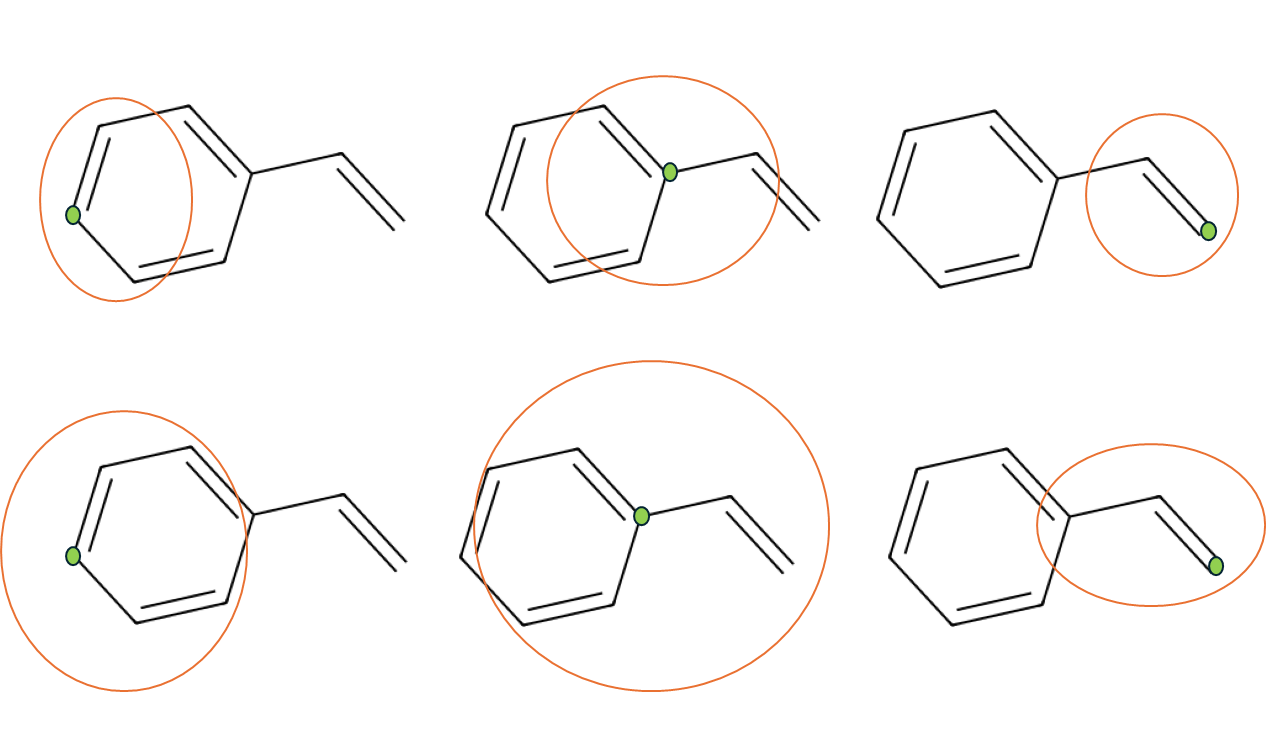
\includegraphics[width=1\linewidth]{morgan_radius.png}
    \caption{radii of selected atoms up to radius 2 for styrene}
    \label{fig:morgan_radius}
\end{figure}


\begin{figure}
    \centering
    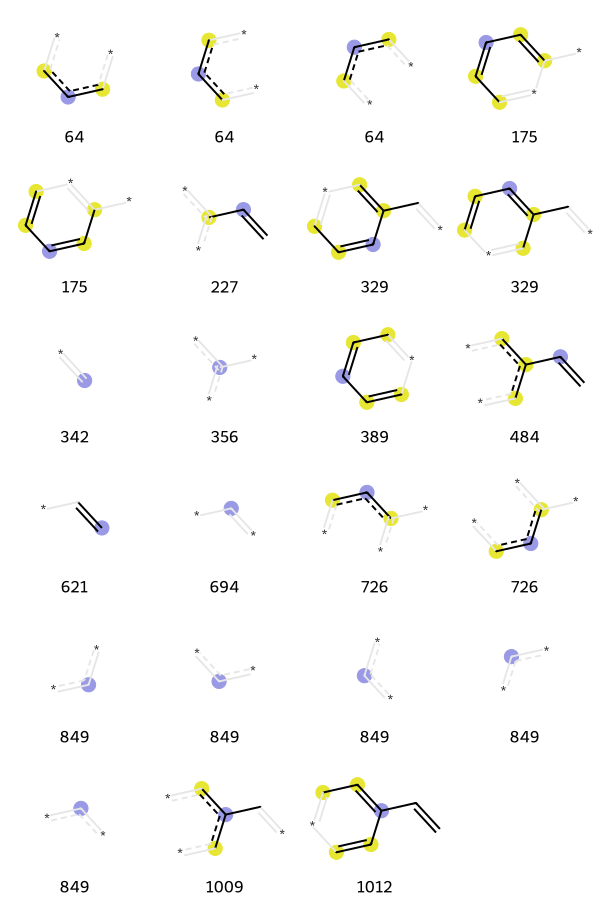
\includegraphics[width=1\linewidth]{styrene_all_subs_morgan.png}
    \caption{all substructures of styrene up to radius 2}
    \label{fig:styrene_all_subs_morgan}
\end{figure}

\begin{figure}
    \centering
    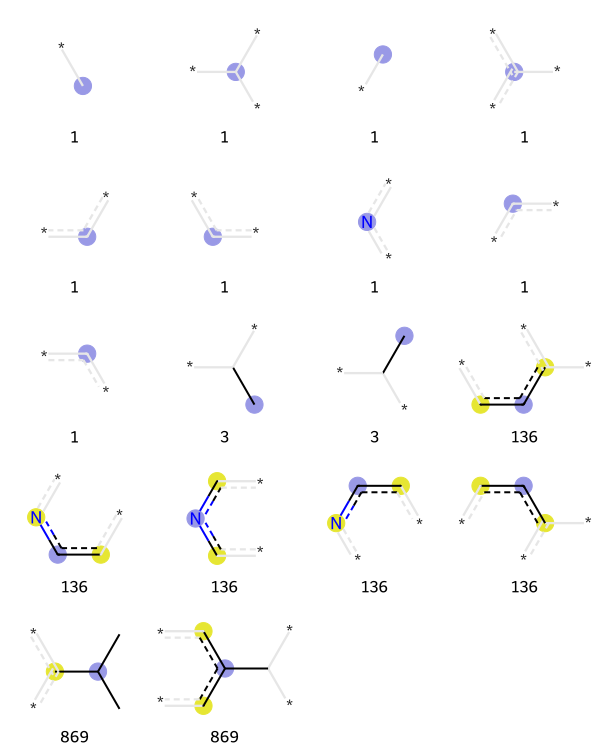
\includegraphics[width=1\linewidth]{substructures_radius1_only_topology.png}
    \caption{Enter Caption}
    \label{fig:substructures_radius1_only_topology}
\end{figure}


\section{Graph Neural Networks}

Graph Neural Networks work on graph data; they can be seen as generalizations of convolutional neural networks (CNNs).

Unlike traditional fingerprints, GNNs treat molecules as graphs, where atoms are nodes and bonds are edges. This structure allows GNNs to directly process the molecular graph and learn more flexible, task-specific representations via message-passing mechanisms. Given that GNNs operate on graph data, they are naturally suited for capturing the intricate connectivity patterns of molecules, which are central to their properties.

They can be applied for different purposes, like node (for individual nodes of the graph, labels or values are predicted)    and graph classification (for the whole graph, a label or value is predicted) as well as link prediction (prediction of the likelihood that an edge exists between specific nodes). In the context of molecular property prediction, one usually deals with graph classification problems, e.g. the label (indicating toxicity, inhibitory activity, etc.) or a value (solubility, lipophilicity, etc.) for the graph which represents a specific molecular compound is determined.

In the following experiments, in particular Graph Convolutional Networks (GCNs) and Graph Isomorphism Networks (GINs) were considered.

It should be noted that there is a much greater variety of GNNs. Some of them, like GATs, yield impressive performance in some tasks.

Most Graph Neural Networks rely on message passing. Different specific architectures are termed MPNN, the central property of the general framework is that a message passing and a readout step are involved. In the context of molecular property prediction, this scheme was introduced in \cite{Gilmer.05.04.2017}.

In the message passing step, each node of the graph passes its feature information to its neighbors and aggregates the information received from them. This process is repeated across multiple layers, allowing each node to gather information from increasingly distant nodes in the graph.

After the graph layer operations, the output has to be arranged in such a way that it can be used for the final prediction, done in the readout step.
Common read-out functions are max and mean; for graph classification and in molecular property prediction, it has turned out that sum is most powerful.

This is usually done using a dense neural network (DNN). (In principle, also a different classifier, e.g. SVM or gradient boost algorithms, could be used; however, for such a set-up backpropagation is probably not feasible. One would have to train the GNN with a simple output layer and after training use the embedding of the GNN as input for the classifier.)

In contrast to Morgan fingerprints, which either provide binary or integer vectors, the GNN architectures usually output a real-valued vector. (Some proposals for creating a representation more similar are proposed below.)

In principle, all GNN architectures suitable for Graph classification can be used for molecular property prediction; however, also some variants like the Attentive Fingerprint are explicitly modeled for this task.

\subsubsection{GCNs}

One of the most commonly used GNN architectures is the Graph Convolutional Neural Network. It can be seen as a generalization of CNNs; whereas the latter can only process input of fixed size, GCNs act directly on the graph representation. As for most graph-based representations, the graph information consists of the adjacency matrix (which in the case of molecule property prediction usually encodes the bonds between atoms) and a feature matrix (which encompasses the physicochemical features of the atoms, e.g. atom type).

Usually, multiple graph convolution layers are stacked. Each layer enriches the represention of a specific node by exploring larger neighbourhoods of the graph. In particular, the first layer aggregates features from the direct neighbours. After this layer, information of the neighbours is stored in each feature representation, so in the next layer also information about the neighbours of the neighbours is incorporated etc.

In the central graph convolution step, neighborhood aggregation is performed: 
\begin{equation}
H^{(l+1)} = \sigma\left(\tilde{D}^{-1/2} \tilde{A} \tilde{D}^{-1/2} H^{(l)} W^{(l)}\right)
\end{equation}


, where W denotes the learnable weight matrix, A the adjacency matrix and D the diagonal degree matrix. \begin{math}\sigma\end{math} corresponds to an activation function, e.g. the often used Rectified Linear Unit activation function (ReLU).


One disadvantage of GCNs is, that they use a mean-based aggregation and this function is not injective. This means that different graphs can lead to the same graph embedding and the network cannot distinguish between the two graphs anymore. One example is visualized in Figure 3 below. Assuming the node and edge properties are identical, GCNs could create the same hidden embedding for these two graphs.

For molecular property prediction, the severity of these limitations relies on several factors (see below); for instance, the occurrence of different, but undistinguishable graphs crucially depends on the used features.

\subsubsection{GINs}

The aggregation function here is a sum.

\cite{Xu.01.10.2018}
GINs (Graph Isomorphism networks) excel in distinguishing different graph structures. It can be shown that they are as expressive as the Weisfeiler Leman algorithm for detecting graph ismorphisms. 
The WL test is determines whether two graphs are isomorphic, i.e. structurally identical, regardless of their labeling.
Thus, if the Weisfeiler Leman algorithm is able to distinguish two graphs, they can also be distinguished by GIN networks. \cite{}


The aggregation function in a Graph Isomorphism Network (GIN) is defined as:

\[
h_v^{(k+1)} = \text{MLP} \left( (1 + \epsilon) \cdot h_v^{(k)} + \sum_{u \in \mathcal{N}(v)} h_u^{(k)} \right)
\]

Where:
\begin{itemize}
    \item \( h_v^{(k)} \) is the feature vector of node \( v \) at layer \( k \),
    \item \( \mathcal{N}(v) \) denotes the set of neighbors of node \( v \),
    \item \( \epsilon \) is a learnable (or fixed) scalar parameter,
    \item \(\text{MLP}\) represents a multi-layer perceptron applied to the aggregated features.
\end{itemize}

The feature aggregation is computed by summing over all neighbours of the node (in principle, also a different aggregation function can be applied, but the sum-function works best for distinguishing graphs).

\( \epsilon \) determines how strongly the node's own features influence the aggregation. It can be implemented as a learnable parameter or set to a fixed value. (Obviously, setting \( \epsilon = 1\), one can eradicate the own features.) 
Similarly to GCN, multiple layers can be stacked to explore the more distant neighbourhood of the graph because at each layer information from the more distant neighours is propagated by feature aggregation.



\subsubsection{GINE}

GINE is an extension of GIN; in contrast to the former, GINE also uses bond information\cite{Hu.29.05.2019}.
This process involves a summation of bond and edge features which requires that the dimensionality of both types of features is identical. (This can be easily attained by adding a preceding linear layer to one type of features with an output layer identical in size to the feature dimensionality of the other feature type, i.e. either for the node or the edges features an embedding with the dimension of the other feature type is created.)



The node update rule for the Graph Isomorphism Network with Edge Features (GINE) is given by:

\[
h_v^{(k+1)} = \text{MLP}^{(k)} \left( (1 + \epsilon^{(k)}) \cdot h_v^{(k)} + \sum_{u \in \mathcal{N}(v)} \text{ReLU} \left( h_u^{(k)} + e_{uv} \right) \right)
\]

Where:
\begin{itemize}
    \item \( h_v^{(k)} \) is the feature vector of node \( v \) at layer \( k \),
    \item \( h_u^{(k)} \) is the feature vector of a neighboring node \( u \) at layer \( k \),
    \item \( \mathcal{N}(v) \) is the set of neighbors of node \( v \),
    \item \( e_{uv} \) is the feature vector of the edge between nodes \( u \) and \( v \),
    \item \( \epsilon^{(k)} \) is a learnable or fixed scalar parameter for layer \( k \),
    \item \(\text{MLP}^{(k)}\) is a multi-layer perceptron for layer \( k \)
\end{itemize}


\subsubsection{GAT}

Graph Attention Networks incorporate information about the neighbourhood of each node by applying a local attention mechanism \cite{Velickovic.30.10.2017}.


Attention scores are computed by introducing a learnable weight vector, e.g.:

e_{ij} = \text{LeakyReLU}\left( \mathbf{a}^\top \left[ \mathbf{W} \mathbf{h}_i \parallel \mathbf{W} \mathbf{h}_j \right] \right)

To obtain normalized attention weights, a softmax function can be applied:



\alpha_{ij} = \text{softmax}_j(e_{ij}) = \frac{\exp(e_{ij})}{\sum_{k \in \mathcal{N}(i)} \exp(e_{ik})}

This attention mechanism should allow to capture long-range dependencies (i.e. influence from more distant nodes) and focus on the most relevant interactions.
The aggregation of the feature vectors of a specific node and its neighbours is weighted by the attention weights.

Graph Attention Networks (GATs) integrate information from the neighborhood of each node by employing an attention mechanism, as introduced in \cite{Velickovic.30.10.2017}. The attention mechanism begins by computing attention scores between node pairs. These scores are determined using a learnable weight vector:

\[
e_{ij} = \text{LeakyReLU}\left( \mathbf{a}^\top \left[ \mathbf{W} \mathbf{h}_i \parallel \mathbf{W} \mathbf{h}_j \right] \right)
\]

To normalize these attention scores, a softmax function is applied, producing attention weights:

\[
\alpha_{ij} = \text{softmax}_j(e_{ij}) = \frac{\exp(e_{ij})}{\sum_{k \in \mathcal{N}(i)} \exp(e_{ik})}
\]

This attention mechanism allows GATs to capture long-range dependencies (i.e., interactions between distant nodes) and to focus on the most relevant connections. The feature vectors of a node and its neighbors are then aggregated, weighted by the computed attention weights:

\[
\mathbf{h}_i^{\text{(new)}} = \sigma \left( \sum_{j \in \mathcal{N}(i)} \alpha_{ij} \mathbf{W} \mathbf{h}_j \right)
\]

In the multi-head attention setting, the updated node feature representation becomes:

\[
\mathbf{h}_i^{\text{(new)}} = \sigma \left( \frac{1}{K} \sum_{k=1}^{K} \sum_{j \in \mathcal{N}(i)} \alpha_{ij}^{(k)} \mathbf{W}^{(k)} \mathbf{h}_j \right)
\]

Here, \( \mathbf{h}_i \in \mathbb{R}^F \) represents the initial feature vector of node \(i\), and \(\mathbf{W}\) denotes a learnable weight matrix. The aggregation process results in the node's new feature representation, \( \mathbf{h}_i^{\text{(new)}} \), after applying the activation function \( \sigma \).

Finally, the loss function used for optimization in GATs is typically defined as:

\[
\mathcal{L} = - \sum_{i \in \mathcal{V}} \sum_{c=1}^{C} y_{ic} \log \hat{y}_{ic}
\]

Different variants exist, e.g. a revised version of the original GAT layer, introduced in \cite{Brody.30.05.2021b}, further improves its performance by addressing some of its limitations.






\subsubsection{Neural Fingerprint}



The Neural Fingerprint, introduced in \cite{Duvenaud.30.09.2015}, was the first graph neural network architecture developed for molecular property prediction. In the experiments presented in \cite{Duvenaud.30.09.2015}, Neural Fingerprints outperformed circular fingerprints, particularly when paired with a linear neural network classification layer on all test datasets. However, the comparisons shown were limited to binary Morgan fingerprints.

A distinctive feature of the Neural Fingerprint is its use of degree-dependent weight matrices. This means that nodes with different degrees are updated using distinct weight matrices. The update rule for node features, as implemented in PyTorch Geometric (see the next chapter), is given by:

\begin{equation}
\mathbf{x}_i' = \mathbf{W}_1^{(\text{deg}(i))} \mathbf{x}_i + \mathbf{W}_2^{(\text{deg}(i))} \sum_{j \in \mathcal{N}(i)} \mathbf{x}_j
\end{equation}



Here, \(\mathbf{x}_i\) represents the feature vector of node \(i\), and \(\text{deg}(i)\) is its degree. The updated features are passed through a sigmoid activation function. Finally, the output is multiplied by learned output weights, and a softmax function is applied to generate the final fingerprint vector. This vector is intially initialized as a zero vector (similar to Morgan fingerprints), and at each layer the contribution from each atom is added to the vector according to the softmax function output.

The Neural Fingerprint shares some conceptual similarities with Graph Isomorphism Networks (GINs). Both architectures aggregate information from the neighbors of a specific node and update the node features accordingly. However, unlike GINs, which use a multi-layer perceptron (MLP) and summation-based aggregation, the Neural Fingerprint uses degree-dependent weight matrices and applies a fixed sigmoid activation function.
In contrast to the processing the sum of the neighbour nodes and self-node update within the MLP, in case of the Neural Fingerprint weight matrices are learnt and a fixed activation function (sigmoid function) is applied.


\subsubsection{Attentive Fingerprint}

The Attentive Fingerprint was proposed in \cite{Xiong.2020} as an extension of the Neural Fingerprint leveraging attention.
In contrast to GCNs and GINs, it also incorporates edge information directly. It extends the idea of the Neural Fingerprint with an attention mechanism similar to that used in GAT. In fact, GAT layers are part of the attentive fingerprint, i.e. it is a specific implementation of this architecture.
The update step in the Attentive Fingerprint shares similarities with the approach used in GCNs, but it integrates attention weights to emphasize the most relevant interactions. These attention weights are computed using a combination of GRU cells and GAT convolutions. 

The implementation provided via PyTorch Geometric uses the original GAT formulation for these convolutions.



\begin{table}[h!]
\centering
\begin{tabular}{|>{\raggedright\arraybackslash}p{3.5cm}|>{\centering\arraybackslash}p{1cm}|>{\raggedright\arraybackslash}p{7cm}|}
\hline
\textbf{Atom Feature} & \textbf{Size} & \textbf{Description} \\
\hline
Atom symbol & 16 & [B, C, N, O, F, Si, P, S, Cl, As, Se, Br, Te, I, At, metal] (one-hot) \\
\hline
Degree & 6 & Number of covalent bonds [0,1,2,3,4,5] (one-hot) \\
\hline
Formal charge & 1 & Electrical charge (integer) \\
\hline
Radical electrons & 1 & Number of radical electrons (integer) \\
\hline
Hybridization & 6 & [sp, sp$^2$, sp$^3$, sp$^3$d, sp$^3$d$^2$, other] (one-hot) \\
\hline
Aromaticity & 1 & Whether the atom is part of an aromatic system [0/1] (one-hot) \\
\hline
Hydrogens & 5 & Number of connected hydrogens [0,1,2,3,4] (one-hot) \\
\hline
Chirality & 1 & Whether the atom is a chiral center [0/1] (one-hot) \\
\hline
Chirality type & 2 & [R, S] (one-hot) \\
\hline
\textbf{Bond Feature} & \textbf{Size} & \textbf{Description} \\
\hline
Bond type & 4 & [single, double, triple, aromatic] (one-hot) \\
\hline
Conjugation & 1 & Whether the bond is conjugated [0/1] (one-hot) \\
\hline
Ring & 1 & Whether the bond is in a ring [0/1] (one-hot) \\
\hline
Stereo & 4 & [StereoNone, StereoAny, StereoZ, StereoE] (one-hot) \\
\hline
\end{tabular}
\caption{Atom and Bond Features Table}
\label{tab:features}
\end{table}


\subsubsection{Higher-order and subgraph GNNs}

Alternatively to the stacking of multiple GNN layers, the incorporation of global information and thus increased expressivity can also be attained via Higher-order GNNs which were propsed in \cite{Morris.04.10.2018}

The concept of Subgraph GNNs is tightly related to Higher-order GNNs.

A recently published type of Subgraph GNN which resembles fingerprints is the Nested GNN \cite{Zhang.2021}. 

However, rooted subtrees have limited expressiveness for representing non-tree graphs. To overcome this, Nested Graph Neural Networks (NGNNs) are proposed, which use rooted subgraphs instead of subtrees.

This approach improves distinguishability between graphs; for instance, many rr-regular graphs, which are not distinguishable by the 1-WL test, have distinct NGNN representations nonetheless.

NGNN works by extracting local subgraphs around each node, applying a base GNN to learn subgraph representations, and pooling these into a whole-graph representation. 


Since all subgraphs are copied to the GPU memory, this approach is - depending, of course, on the available resources - only feasible for rather small graphs (as it is typical for molecular graphs).

Similarly, for Nested GNNs high variance was reported in \cite{Zhang.2021}. They trained for a fixed number of epochs. In addition to the final model, every 10 epochs a checkpoint was created, and the average ensemble performance was also reported.

Each subgraph up to a specific radius is evaluated; as base GNN various architectures, e.g. GCN and GIN, can be used.
In \cite{Zhang.2021}, this architecture was tested on the QM9 dataset and the HIV and PCBA datasets.



\subsection{Combination of fingerprint and GNN information}

Meanwhile, it was also explored whether the combination of molecular fingerprint and graph-based representations can improve predictive power. A simple approach computes both separately and passes both outputs to a final classifier (e.g. a dense neural network layer, but also a different architecture depending on the task would be possible).

In \cite{Zhang.2024}, several different fingerprints were computed and a feature selection module created a reduced version by maximizing relevance and minimizing redundancy. 

Similar to \cite{Zhang.2024}, fingerprint and GNN information was also combined.


In \cite{Liu.2025}, a model called fingerprint-enhanced hierarchical graph neural network (FH-GNN) is proposed.
On eight benchmark datasets from MoleculeNet, it outperformed many baseline models and competitors.  


In many cases, results are ambiguous. For example, the complex graph-based architecture proposed in \cite{Yang.2019} achieved superior results on some datasets, but on other it performed equal or even worse than a Random Fores classifier applied on fixed molecular fingerprint representations.

Another approach uses fragmentation methods like BRICS to obtain processable, chemically or archaeologically meaningful substructures of a molecule \cite{Degen.2008,Jinsong.2024,ZhangBRICS.2024,Liu.2017,Diao.2023}.


\subsection{More complex architectures for molecular property predictions}


In \cite{Alon.09.06.2020}, an additional fully adjacent layer (in which all nodes are connected) was applied in order to attenuate bottleneck effects.

For example, \cite{Liu.2025} and \cite{Zang.2023} use the BRICS algorithm to create fragments for a hierarchical molecular graph.


or hierarchical molecular graph neural networks (HimGNN) \cite{Han.2023}, which applies a Transformer architecture to fuse atom- and molecular motif-based graphs.

Hyper-Mol creates a molecular graph representation based on the preceding extraction of ECFP fingerprints \cite{Cui.2023}.

A message passing algorithm using bond information (instead of the usual node based message passing), termed directed MPNN (D-MPNN), was proposed in \cite{Yang.2019}. This message passing scheme is directed in such a way that the messages at the current step are not influenced by the message in the reverse direction from the previous step, attenuating the problem of tottering.


Bitwise and Count fingerprints were also used as baseline in \cite{Yang.2019}. For some datasets, similarly large differences were found, but not in all; a plausible explanation is different, and possibly insufficient, hyperparameter optimization. Indeed, it is noted in \cite{Yang.2019}, that all architectures (baseline as well as the newly proposed D-MPNN) are applied with unspecified default parameters (making a fair comparison virtually impossible, see results and discussion section).

Another approach features data augmentation and contrastive learning \cite{Wang.2022} .Motif-driven contrastive learning is also applied in \cite{Zhang.2024b} and multiple molecular graph representations of different granularity are combined in \cite{Kengkanna.2024}.

Another self-supervised pre-training scheme was proposed in \cite{Wan.2025}. In \cite{Wan.2025}, also performance in the presence of activity cliffs was studied in more detail. Similarly DGCL, uses a similar combination of two GNNs (GIN and GAT) and additionally incorporates fingerprint information \cite{Jiang.2024}. The version with both GNNs was compared to architectures consisting of ECFPs combined with pre-trained GIN and GAT layers. These combinations improved performance on some datasets (however, unfortunately, the ECFP baseline was not checked, so it is difficult to fully assess the performance gain).

Other graph-based approaches apply self-supervised learning. For instance, GROVER (Graph Representation frOm self-superVised mEssage passing tRansformer), a transformer-based framework with 100 million parameters, which was pre-trained on 10 million unlabelled molecules \cite{Rong.2020}, is widely used.

Similarly, MolBERT is a BERT model pre-trained on four million unlabeled compounds which can be used for  molecular property prediction tasks \cite{Li.2021}. Interestingly, as shown in the discussion below in more detail, even these large models do not persistently outperform simpler GNN architectures or even ML classifier acting on Morgan fingerprints.

\section{Activity cliffs}

Recently, in the context of QSAR, the role of activity cliffs is intensively discussed. Such activity cliffs consist of molecules which are structurally very similar, but feature highly different molecular properties.

This implies that the structural differences cause big biological differences.\cite{Stumpfe.2019} It is crucial to not confuse them with outliers \cite{Maggiora.2006}.

In particular, it is astonishing that molecular fingerprints outperform GNNs especially in ‘difficult’ tasks which should be more suited for the latter, e.g. in activity cliff prediction.

Also \cite{Jiang.2021} rightly mentions that these evaluations are often rather biased against the classical fingerprints. For example, for ECFP only Random Forests and Support Vector Machines are tried as classifiers, but newer, more complex and potentially superior ML classifiers, e.g. gradient-boosting techniques like LightGBM, are not included in the benchmark. In many cases, also hyperparameter optimization can lead to performance distortions which are wrongly interpreted as essential differences between the architectures. 


\section{Previous work}

Similarly, in \cite{Jiang.2021} classical fingerprints in combination with a DNN or a classical ML algorithm (e.g. support vector machines or random forests) outperformed graph-based models in most tasks. Only for some larger and multi-task datasets graph representations yield better performance than the descriptor-based models, implying that data availability is critical. (However, studies systematically evaluating the impact of additional data on specific datasets are largely missing.)
The graph models investigated in \cite{Jiang.2021} were GCNs, attentive FP and a MPNN model; GIN was not applied.

Graph-based models show better performance only on larger dataset.
SVM generally achieves the best predictions for the regression tasks. Both RF and XGBoost can achieve reliable predictions for the classification tasks, and some of the graph-based models, such as Attentive FP and GCN, can yield outstanding performance for a fraction of larger or multi-task datasets. In terms of computational cost, XGBoost and RF are the two most efficient algorithms and only need a few seconds to train a model even for a large dataset. The model interpretations by the SHAP method can effectively explore the established domain knowledge for the descriptor-based models.
 
On the HIV dataset, it was shown that different classifiers yield different profiles.

In \cite{Dablander.2023}, the performance of ECFPs and other descriptors is compared to GINs on several binding affinity data sets with a focus on activity-cliff prediction. The authors state that activity cliffs seem to be a major problem for accurate predictions and, on average, graph-based representation cannot handle them more efficient than the simpler fingerprints. 

Similarly, \cite{Stepisnik.2021} state that deep learning approaches do not yield better performance compared to classical fingerprints in spite of their much higher computational cost.

In the same vein, \cite{Deng.2023} stresses the importance of activity cliffs.

Moreover, in some cases, circular fingerprints coupled with a classical ML method, e.g. support vector machines, outperformed a DNN version. Again, this was the case in a study focusing on activity cliffs using CHembl.

However, it should be noted that most of these studies show serious flaws or gaps (which will become even more obvious regarding the results of this investigation).

In \cite{Jiang.2021}, the models were evaluated on 50 random splits. Although one could argue that the comparatively high number of runs cover a wide range of possible combinations, this procedure does not substitute for other splits.
Moreover, hyperparameter optimization only processed a small list of possible values for parameters like the hidden channel size within a limited range, possibly reasonable parameter combinations were missing; for continuous variables like the learning rate only a few possible values were assigned. Furthermore, techniques like normalization layers were not considered (dropout was only a parameter for the final prediction layer). 


However, a meta-analysis of the results is hardly possible because often the indication of crucial parameters is missing. For instance, it is not always clear which atom and node features have been used (it can be assumed that likely the default featurizer of the used GNN framework was applied; since many frameworks have specialized featurizers for specific architectures, it is even more difficult to decide). Hence, it could be necessary to evaluate the impact of such factors.

In the same vein, the Attentive FP, i.e. the application of GAT to molecular property prediction, proposed in Xiong et al. 2020 showed superior performance in almost all tasks from MoleculeNet. However, only three runs were performed and for regression tasks like ESOL solely random splits were applied. Furthermore, as in \cite{Duvenaud.30.09.2015}, it seems that the ECFP used only bitwise features which leads to much worse performance of the fingerprint.

For the regression tasks, mostly the random split is used. Furthermore, for the classification tasks of MoleculeNet, except for the MUV-dataset, usually ROC-AUC is used as metric, although all datasets are rather imbalanced (e.g. in \cite{Zhang.2024}). In particular, it should be noted that for scaffold splits the imbalance can be much higher than for the complete dataset, hence leading to a potentially misleading ROC-AUC.

It is also problematic that sometimes error estimates (e.g. in \cite{Zhang.2024}) are missing, which makes the ranking of the classifiers in case of small differences (or possibly high inter-run variances) impossible.

Similarly, in \cite{vanTilborg.2022}, all models were trained for 300 epochs and the early stopping patience was set to ten epochs, which arguably is a very low number in this setting (especially given the fact that most datasets are not very big), possibly excluding good solutions.

High inter-run variance as well as small parameter deviations probably explain that results often cannot be replicated.
For instance, in \cite{Zhang.2024}, a new hybrid fingerprint-GNN approach is presented and compared against other algorithms like Attentive FP. 
In the original publication, for ESOL, FreeSolv and lipophilicity, values of 0.503, 0.736 and 0.578 were reported; the evaluation of Zhang provided 0.587, 1.091 and 0.553.

These issues are extensively discussed in \cite{Wallach.2018}

Furthermore, the inference from low p-values (without accompanying effect sizes) that there is a significant effect is correctly criticized given the fact that for increasing sample size (which can be arbitrarily increased by evaluating a higher number of test splits) p-values get arbitrarily low. \cite{Robinson.2020} 

It should be noted that protein-ligand and ligand-ligand interaction tasks often provide spurious results \cite{Volkov.2022}.
Even when it is unlikely due to these problems that one gets results sufficiently reliable for practical application, the comparison between circular fingerprints and GNNs could also be insightful in this case.



\section{Potential Pitfalls and Limitations}

Over-fitting, over-smoothing, and over-squashing represent significant challenges to the performance of Graph Neural Networks (GNNs) \cite{JunXia.2023}.

Fundamental limits of expressivity, i.e. there are graphs which cannot be distinguished by GNNs working with the message passing paradigm, have also to be taken into account. However, since in most molecular property prediction tasks the central goal is not to have a unique mapping of each molecule, but a representation which allows an accurate prediction of the objective value. (In principle, for a binary classification task it would be sufficient to map all input graphs to two different output vectors.)


Over-smoothing occurs predominantly in models with stacked graph layers. After several layers, node embeddings tend to converge to similar values, which diminishes the ability of the model to differentiate between nodes and often leads to degraded performance. This is highly problematic in the context of molecular property prediction.


Over-fitting is particularly challenging in molecular property prediction tasks. This issue stems from two main factors: Firstly, there is often a limited availability of training examples, and, exacerbating the problem, data is often highly imbalanced. Secondly, one has to consider substantial differences between training and test examples, which make over-fitting to the training data especially detrimental.

Over-squashing arises when the graph topology creates a bottleneck for message propagation, distorting the flow of information. While this phenomenon can severely affect certain graph types, it is generally less problematic for smaller graphs, such as those commonly used in molecular applications.

\cite{CortesCiriano.2019} used Morgan Fingerprints with a comparatively small size (128) as input for DNN and RF ensembles, reporting that larger fingerprint sizes did only marginally improve results. In this publication, another technique called snapshot ensemble learning is introduced \cite{CortesCiriano.2019}. The training process is divided into cycles and after each converged cycle the learning rate is set back to its original value.

Furthermore, in the creation of datasets like HIV and the toxicity-related ones, a threshold for obtaining binary classification labels was applied. This allows that there are very similar molecules in terms of the original value, which are artificially separated into two different groups due to the threshold.




In \cite{TranNguyen.2020}, where the LIT-PCBA dataset is presented, these problems are well summarized:
'Intriguingly, DNNs trained with rigorous crossvalidation procedures on simple ligand descriptors were almost as accurate as those trained on protein−ligand attributes, evidencing that deep learning did not learn anything about the physics of protein−ligand interactions. Strikingly, the literature is full of overoptimistic reports describing machine learning models with near perfect performances on the above described data sets, although true VS practitioners have known for a long time that such an accuracy level does not mirror the proportion of experimentally confirmed hits in real prospective VS experiments.' \cite{TranNguyen.2020}


Moreover, most GNN architectures have been introduced with very specific parameters. For instance, in the AttentiveFP paper it is not taken into account that also the selection of node and edge features (which differs strongly from other set-ups) could be responsible for the performance gain (and not the newly proposed architecture itself).
	\chapter{Molecular property prediction}

Furthermore, usually it is only stated that there are different results on different data size, but an explanation or at least an investigation of the correlation between training set size and performance is missing.

\section{Regression tasks}

For regression tasks, MAE and MSE are used as loss functions. For the predictions, both errors are reported. 
Given the potential role of outliers, it seems advisable to compare both errors.

\section{Classification tasks}

For classification tasks, AUPR and AUROC are reported. For specific cases of interest, precision-recall curves are shown.
Furthermore, the distribution of predicted probabilities is investigated.

\section{Protein - ligand and ligand -ligand interaction}

It should be noted that protein-ligand interaction tasks often provide spurious results \cite{Volkov.2022}.
Even when it is unlikely due to these problems that one gets results sufficiently reliable for practical application, the comparison between circular fingerprints and GNNs can be highly insightful.

\section{Datasets}


One of the most widely datasets for molecule property prediction is MoleculeNet \cite{Wu.2018}. There are, however, several intricacies which potentially thwart MoleculeNets role as unbiased measure of model performance.

Pytorch Geometric and DGL support direct access to the MoleculeNet datasets.
Modified versions of the MoleculeNet datasets are also provided by the Open Graph Benchmark \cite{Hu.02.05.2020}. 

In the Open Graph Benchmark paper \cite{Hu.02.05.2020}, GINs and GCNs were compared on two of the MoleculeNet datasets. For GINs, versions with additional virtual nodes performed best.
However, in this evaluation benchmark, a rather peculiar configuration has been chosen (5 GNN layers with 300 hidden channels and average pooling function); so, again, it is likely that the ranking of the models would be different for other (and perhaps superior) hyperparameter settings.

The benchmark on two MoleculeNet datasets in the Open Graph Benchmark paper \cite{Hu.02.05.2020} also showed big differences between random and scaffold splitting. Furthermore, it was claimed that different libraries give rise to scaffold splits of different difficulty (the version for the preprocessing of the Open Graph Benchmark datasets being the most diffcult one, maximizing diversity between train and test data). 



\subsubsection{ESOL}

The ESOL dataset consists of 1128 common small organic molecules for which water solubility data (log solubility in mols per litre) was determined. \cite{Delaney.2004}

\cite{Delaney.2004} also derived a regression formula for the solubility (since then, various more advanced versions have been conceived) from global molecular properties:
\[
\log(S_w) = 0.16 - 0.63 \cdot \text{clogP} - 0.0062 \cdot \text{MWT} + 0.066 \cdot \text{RB} - 0.74 \cdot \text{AP}
\],
with clogP the logarithm of the octanol-water partition coefficient, MWT the molecular weight, RB the number of rotatable bonds and AP the aromatic proportion, i.e. the proportion of heavy atoms in the molecule which participate in an aromatic ring.


\subsubsection{FreeSolv}

The FreeSolv dataset consists of 1128 the hydration energies of 644  small organic molecules. There are experimental values as well as data calculated by alchemical free energy simulations.
\cite{Mobley.2014}


\subsubsection{Lipophilicity}

curated from ChEMBL database,45 provides experimental results of octanol/water distribution coefficient (log[thin space (1/6-em)]D at pH 7.4) of 4200 compounds
Experimental results of octanol/water distribution coefficient(logD at pH 7.4).

\subsubsection{HIV}

The task is to predict the ability of molecules to inhibit HIV replication.
It consists of 41127 molecules which were evaluated during 47 screening results were evaluated and placed into three categories: confirmed inactive (CI), confirmed active (CA) and confirmed moderately active (CM).
The binary positive class is merged from 'moderately active' and 'active'. (It would be reasonable to only retain the positive instances originally labeled as 'active'; however, usually the full dataset is processed.)





\subsubsection{BACE}


The BACE binding provides bindings results for a set of inhibitors of human beta-secretase (BACE-1). BACE-1 is involved in the formation of myelin sheaths and also in β-amyloid formation which is supposed to be responsible for Alzheimer's disease.
It consists of 1124 instances. It contains data for a regression task (IC50-values), but usually the binary labels (inhibiting/not-inhibiting) are used for a binary classification task.


\subsubsection{BBBP}

THE BBBP dataset contains data from modeling the blood–brain barrier (BBB) penetration of compounds which is a crucial property in the development of new drugs. It is a binary classification task which distinguishes between molecules which cannot penetrate (negative class) and which penetrate the blood-brain barrier.

\subsubsection{ClinTox}

The ClinTox dataset provides information about drug toxicity. It comprises drugs approved by the FDA and drugs that have failed clinical trials due to toxicity. It is a binary classification task, containing 1491 drugs and their toxicity as well as their FDA approval status. 

\subsubsection{ZINC}

The ZINC database provides comprehensive information 
For the used dataset, the goal is to predict the constrained solubility of the molecules
The full set consists of 250k molecules.
Fig. \ref{fig:zinc_descr} shows the distribution of the molecular weight and the solubility of the full dataset.
As the dataset from pytorch Geometric does not contain SMILES-strings, the ZINC dataset from the deepchem library was used.
In the context of this study, the enormous size of the ZINC dataset allows for a systematic investigation of the influence of the training data size on the performance of GNNs.

\begin{figure}
    \centering
    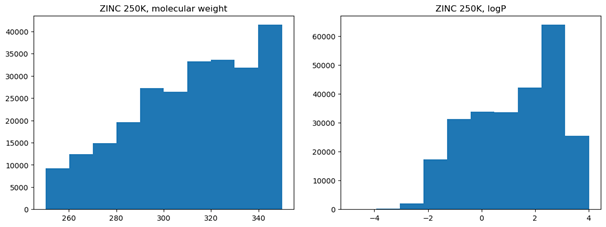
\includegraphics[width=0.75\linewidth]{zinc_descr.png}
    \caption{Enter Caption}
    \label{fig:zinc_descr}
\end{figure}

\subsubsection{ADME}

The ADME (absorption, distribution, metabolism, and excretion) dataset consists of 3521 diverse compounds which belong to 3028 distinct scaffolds. 2736 of these scaffolds contain only one molecule \cite{Fang.2023}. This should ensure a very high structural diversity (and make scaffold splitting rather unnecessary, see chapter methods). 
ADME processes ; for potential drug candidates a balanced ADME profile is an essential property \cite{Fang.2023}.
Six properties are given: include human liver microsomal (HLM) stability reported as intrinsic clearance (Clint, mL/min/kg), MDR1-MDCK efflux ratio (MDR1-MDCK ER), solubility at pH 6.8 (ug/mL), rat liver microsomal (RLM) stability reported as intrinsic clearance (Clint, mL/min/kg), human plasma protein binding (hPPB) percent unbound, and rat plasma protein binding (rPPB) percent unbound.

For example, in \cite{Fang.2023} it is noted that the addition of 2D RDKit descriptors to the molecular graph representation improved the performance. 


Unfortunately, for two of the six properties the number of molecules for which information is available is very small. For the other properties, especially for solubility, the values are highly skewed (fig. \ref{adme_value_distribution}.

\begin{figure}
    \centering
    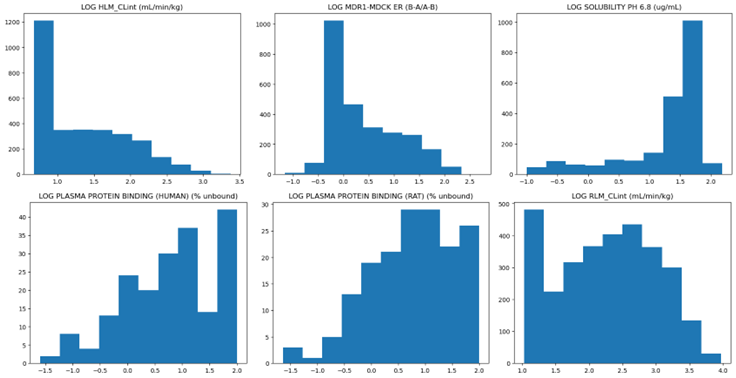
\includegraphics[width=1.1\linewidth]{adme_value_distribution.png}
    \caption{Distribution of the objective values in the ADME dataset}
    \label{fig:enter-label}
\end{figure}

\begin{table}[ht]
\centering
\begin{tabular}{|>{\raggedright\arraybackslash}p{5cm}|>{\raggedleft\arraybackslash}p{3cm}|}
\hline
\textbf{Total Molecules in dataset} & \textbf{3521} \\ \hline
\textbf{LOG HLM\_CLint (mL/min/kg)} & 3087 \\ \hline
\textbf{LOG MDR1-MDCK ER (B-A/A-B)} & 2642 \\ \hline
\textbf{LOG SOLUBILITY PH 6.8 (ug/mL)} & 2173 \\ \hline
\textbf{LOG PLASMA PROTEIN BINDING (HUMAN) (\% unbound)} & 194 \\ \hline
\textbf{LOG PLASMA PROTEIN BINDING (RAT) (\% unbound)} & 168 \\ \hline
\textbf{LOG RLM\_CLint (mL/min/kg)} & 3054 \\ \hline
\end{tabular}
\caption{Data table of different properties}
\end{table}

\begin{figure}
    \centering
    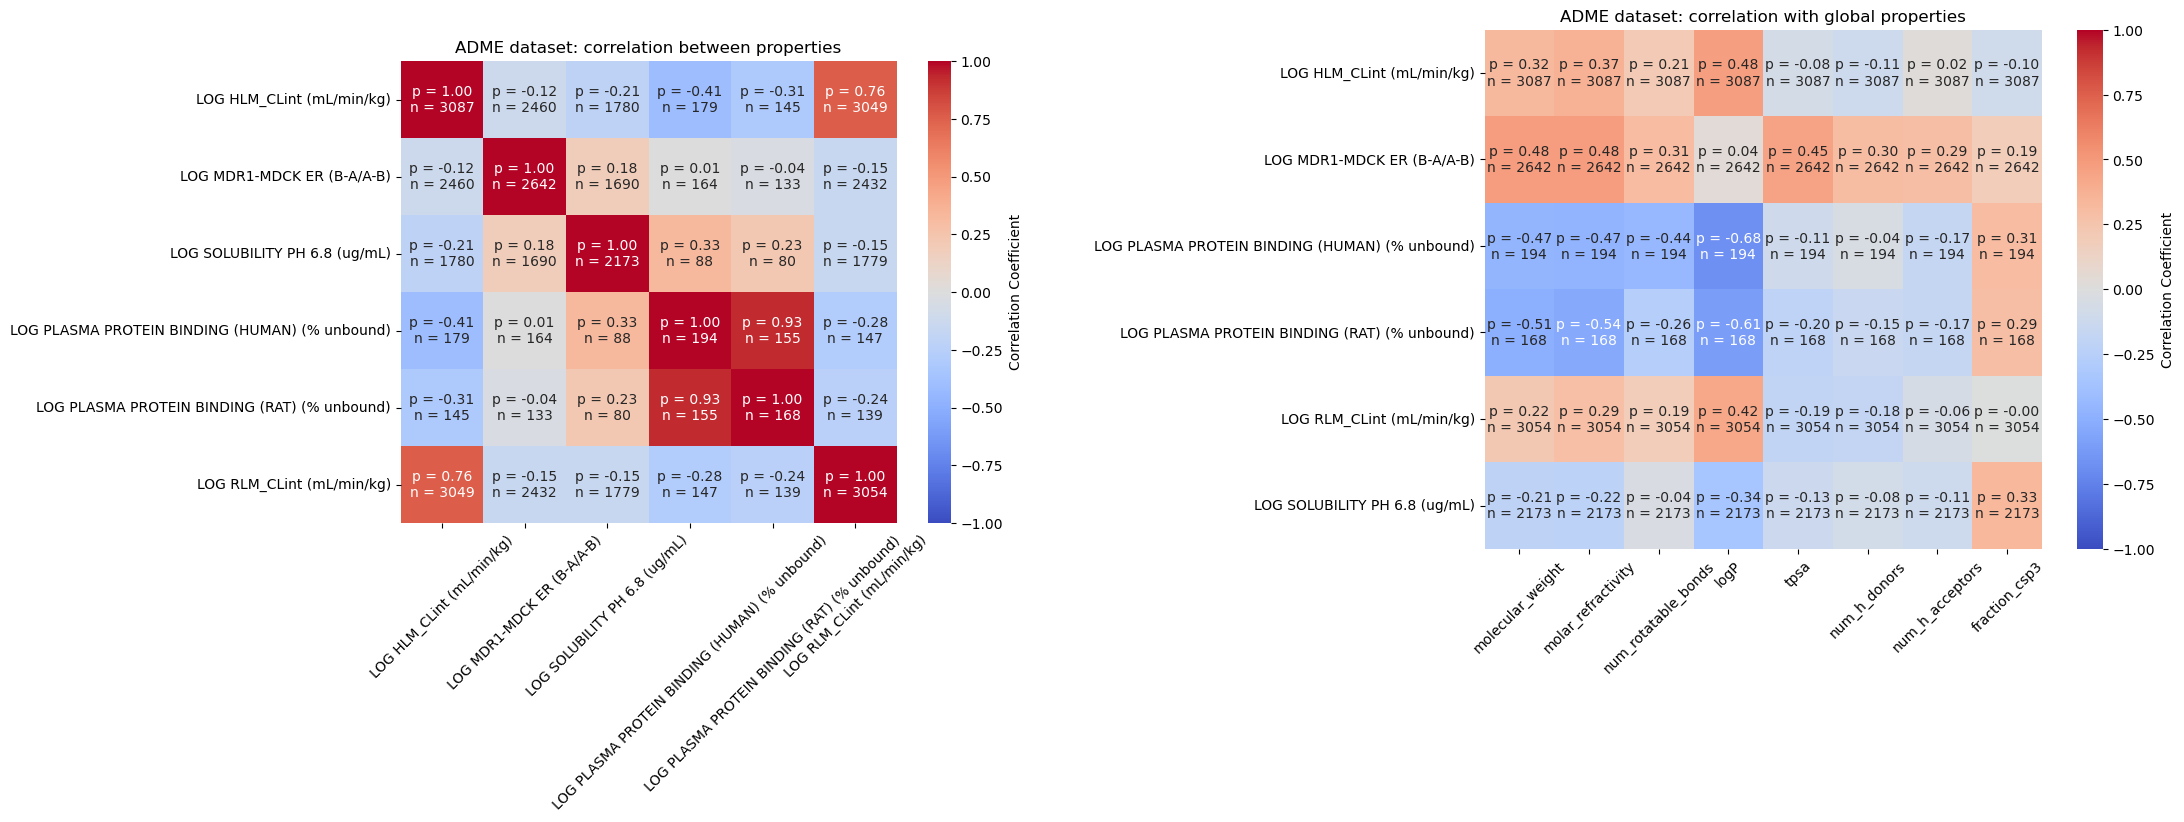
\includegraphics[width=1\linewidth]{adme_correlations.png}
    \caption{Enter Caption}
    \label{fig:enter-label}
\end{figure}

\subsubsection{Cancer data from NCBI}


\cite{He.2021} constructed a phenotypic screening data set comprising 13 breast cancer cell lines and one normal breast cell line.
The data was analyzed with with multiple GNNs, including a hybrid incorporating information from multiple fingerprint representations, but not the usual Morgan fingerprints.


In \cite{HernandezHernandez.2023} tested clustering approaches on data from the NCI-60 cancer cell line panel. was analyzed using graph representations.
\cite{Guo.2024} 
One of the examples investigated in this thesis is IGROV-1, a well-established cell line which acts as a model for drug-resistant ovarian carcinoma exhibiting low to moderate sensitivity to several common chemotherapeutic agents. \cite{Guo.2024} 



\subsubsection{LIT-PCBA}


The LIT-PCBA dataset aims to provide an unbiased dataset for machine learning and virtual screening. It consists of entries of bioactivity data from the PubChem BioAssay database (PCBA). 
It consists of 15 targets, 7844 active, and 407381 inactive compounds\cite{TranNguyen.2020}. The data set encompasses information from 149 dose-response PubChem bioassays. Properties like molecular weight are within a similar range for active and inactive compounds. False positives and assay artifacts were removed. All examples in LIT-PCBA are extremely imbalanced. For most proteins, only a few active compounds are given. This ratio mimics the setting of experimental screening.
Examples are the TP53 Cellular tumor antigen p53 inhibitor (602 actives, 10488 total) and the Estrogen receptor β antagonist (477 actives, 10486 total).

The corresponding ligand sets were unbiased by the asymmetric validation embedding (AVE) procedure. AVE systematically measures the pairwise distance in chemical space between molecules belonging to four sets of compounds. Since the unbiasing is based on ECFP4 fingerprints, one could assumed that it is ‘biased’ against the Morgan fingerprints.


\subsubsection{Activity data from ChEMBL}


A further activity dataset was proposed in \cite{CortesCiriano.2019}. It contains data from ChEMBL concerning the inhibition of diverse molecular compounds like the neurotransmitter dopamine, estrogen and the protein HERG which acts as a potassium ion channel. These molecular compounds are of great interest for drug discovery; e.g., inhibition of hERG is a side-effect of some drugs, leading to severe heart failure. 
In a similar vein, an opioid-related dataset from ChEMBL was assembled for benchmarking in \cite{Deng.2023}. It includes K-related targets like multi-drug resistance protein 1 (MDR1), cytochrome P450 2D6 (CYP2D6) and CYP3A4. Relevant PD-related targets include the μ-opioid receptor (MOR), δ-opioid receptor (DOR), and κ-opioid receptor (KOR).
In \cite{Deng.2023}, only classical fingerprint models and pretrained models like Grover and MolBERT were applied on these datasets. Fingerprints were never outperformed, but for smaller datasets they were much better than pretrained transformer models (for small data, MolBERT was worst by far). In the following, it will be investigated how graph representations perform on these datasets.

Two examples from the dataset are the neurotransmitter dopamine and hERG, the alpha subunit of a potassium ion channel essential for cardiac function, whose binding by drugs can lead to adverse side effects.

The selection investigated in this thesis was chosen in such a way that it provides a rather diverse subset, e.g. concerning data size as well as function, and allows, if possible, a direct comparison with the results in the publication it was firstly used. For example, IGROV-1 was presented as paradigmatic example in \cite{Zhang.2024}.


	\chapter{Methods}

\section{Basics}

\subsection{GNN libraries}

\subsubsection{Pytorch Geometric}

Pytorch Geometric provides the most common GNN models, e.g. GCNs and GINs. These types are usually implemented in two versions.
Pytorch \cite{Paszke.03.12.2019}

\subsubsection{DGL}

The DGL Model Zoo encompasses many GNN architectures for molecular property prediction, including neural versions of fingerprints (currently: AttentiveFP Predictor, GAT Predictor, GATv2 Predictor, MGCN Predictor, MPNN Predictor, SchNet Predictor, Weave Predicot, GIN Predictor, GNN OGB Predictor, Neural Fingerprint Predictor, Path-Augmented Grpah Transformer Predictor).

\subsubsection{PyGHO}

Pytorch Geometric Higher Order (PyGHO) provides models and appropriate data structures for Higher-Order GNNs \cite{Wang.28.11.2023}.

It should be noted that, in contrast to Pytorch Geometric and DGL, this recently published library was not heavily used until now; thus it cannot be ascertained that the implementations are fully correct and actually represent the proposed models.

\section{Evaluation and analysis}

\subsection{Tanimoto similarity}

Tanimoto similarity is a commonly used metric for assessing the similarity between molecular compound.
The general formula is equivalent to Jaccard similarity and given by
\[
\text{Tanimoto / Jaccard Similarity} = \frac{|A \cap B|}{|A \cup B|}
\]


In a first step, the Morgan fingerprint of the molecules of interest is computed.
(It should be noted that the settings for the Morgan fingerprint can influence the results, especially a fingerprint size set much too small leading to collisions.) Afterwards, the similarity between the two fingerprint vectors is calculated.





In \cite{Duvenaud.30.09.2015}, the following generalization for continuous data is used for comparing neural and classical circular fingerprints:
\[
\text{distance}(x, y) = 1 - \frac{\sum \min(x_k, y_k)}{\sum \max(x_k, y_k)}
\]


\subsection{Metrics}



\subsubsection{Regression tasks}

The most commonly used loss functions are MAE and MSE loss, for the error of the final prediction either RMSE, 

\begin{equation}
\text{RMSE} = \sqrt{\frac{1}{n} \sum_{i=1}^{n} (y_i - \hat{y}_i)^2}
\end{equation}
and MAE, 
\begin{equation}
\text{MAE} = \frac{1}{n} \sum_{i=1}^{n} |y_i - \hat{y}_i|
\end{equation}
is used.
This could be of interest for the tasks since often outliers influence the results dramatically.


\subsubsection{Classification tasks}


For benchmarking of the molecular tasks, often AUROC is used. However, due to the imbalance of most datasets, its usage has also been rightly criticized (\cite{Robinson.2020}) as misleading (at least when it is used as performance benchmark without combination of other metrics).

In the following experiments for classification tasks primarily AUPRC is used.

Precision or positive predictive value (PPV) is defined as
\begin{equation}
\text{Precision} = \frac{\text{True Positives}}{\text{True Positives} + \text{False Positives}}
\end{equation}

\begin{equation}
\text{Recall} = \frac{\text{True Positives}}{\text{True Positives} + \text{False Negatives}}
\end{equation}

Alternatively, in \cite{Jiang.2021}, positive predictive (PPV), i.e. precision, in combination with negative predictive value (NPV),

\begin{equation}
\text{NPV} = \frac{\text{True Negatives}}{\text{True Negatives} + \text{False Negatives}}
\end{equation}
, is recommended.


Since PPV and NPV require a pre-defined threshold, it seems that AUPRC is most convenient for comparing the performance across different architectures.

    \chapter{Implementation details}


For this purpose, highly customizable workflows based on PyTorch have been implemented.


Furthermore, some basic notions which are of particular importance for the performance of the architectures, e.g. norm layers, will be explained in some more detail.

Furthermore, 'molecules' with less than two atoms were discarded. (Certainly, this does not make any difference because usually in the datasets there are only proper molecules; however, in some cases, defective SMILES led to such entries.) 

So in a first step, for multiple datasets (see tasks, datasets) provisional results were computed and it was checked whether significant differences between approaches and architectures can be found.

For most architectures and parameter settings, the first benchmarks were performed using the simple, often used ESOL dataset. Given the results on this dataset, selected methods were investigated in more detail on other datasets.

If not stated otherwise, the datasets were not preprocessed, e.g. no outliers or duplicates were removed.



higher-order

The evaluation of such a network architecture is also interesting for comparison purposes since they were not tested on molecular graphs except for the ZINC dataset in the Nested GNN publication (In the format of the default ZINC loader from Pytorch Geometric with solely the atom type as atom feature).

The only used feature was the atom type.
(In the format of the default ZINC loader from Pytorch Geometric). (In principle, it should be easy to project lists of features to 1D.)


In this regard, one would also have to reflect what constitutes a fair comparison: For GNNs – given sufficient input data as well as neuron and layer numbers -, it is rather natural that additional information, e.g. additional node features, increase the performance (as long as it is really additional information about the underlying distribution and not just noise).



\subsection{Further implementation details}

On several occasions, this required the implementation of the models with different libraries.
In particular, additional runs can be started and, upon completion, will be automatically added to the analysis pipeline.
Either optuna hyperoptimization is performed and subsequently a run with the optimized parameters is performed, or manually set parameters can be used.
Additionally, it was also implemented to use other classifiers for the fingerprints as DNNs, e.g. SVMs and Gradient Boost methods like LightGBM.

For optimization a multi-step approach was chosen: Given the amount of data sets, splits, parameters, architectures and possible feature combinations, it would be infeasible to run hyperparameter optimization for every reasonable setting.
In a first step, for all datasets hyperparameter optimization for the models of main interest (GCN, GIN, Morgan fingerprint with bitwise- and count-features and, for some some datasets, Neural Fingerprint) was performed with default settings (for instance, the default atom and bond features) and deactivation of additional, possibly performance-increasing architectural features like normalization and dropout layers.

Afterwards, the optimal hyperparameters determined have been used for extended experiments, for instance using different atom features or jumping knowledge.

In cases of promising results - i.e. when without new determination of optimal hyperparameters the results were better, e.g., in terms of mean error or variance of the error -, hyperparameter optimization was performed anew for these settings.

Unfortunately, for these classification tasks in almost none publication it is revealed how this data imbalance is tackled (which suggests that the data is taken as it is). Given the fact that most typical benchmark datasets (e.g. from MoleculeNet) are highly imbalanced, this is very problematic. It turns out to be even more severe since many split techniques, e.g. the usually, in addition to the random split, applied scaffold split, leverages the imbalancing extremely.
Common ways of treating imbalanced datasets are upsampling, i.e. instances of the rare class are copied, and weighting, i.e. the errors/losses get weighted proportional to their frequency in the dataset.



\subsection{Data splits}

Alternatively to random splitting, one can apply scaffold splitting \cite{Bemis.1996}.
The assumptions of the reasoning behind the scaffold split are not always met: Firstly, it could be…
On the other hand, it could be that a totally different mechanism is responsible for activity or toxicity in another compound; it is obvious that such generalization can be extremely difficult or even impossible. 

Scaffold splitting explores the difficulties of predictors in dealing with inter-scaffold generalization, whereas activity cliff prediction affords intra-scaffold generalization. \cite{Deng.2023}

A straightforward idea for splitting is to directly use similarity information, e.g. obtained by Tanimoto similarity.


Given the high correlation between molecular weight and a multitude of properties, e.g. solubility, such a weight split often also entails a split with regard to the objective value.
It should be noted that the MolecularWeightSplitter of the DeepChem- and of the DGL-library are fully deterministic and does not depend on the ordering of the input data, i.e. shuffling does not change the output of the splitter. 

The DeepChem TaskSplitter tries to split the datasets as evenly as possible with regard to the objective value (i.e., for classification tasks, the proportion of all sets generated by the split should be as equal to the original input as possible, and for regression tasks, the same holds for the distribution of the values to be predicted).

The DGL SingleTaskStratifiedSplitter can also be used.


Given the main difference between the Graph representations and the fixed-size fingerprints, namely that the former can specify due to their learnable weights to a specific task, the results for the Task splitting, in which splitting is done so that batches with a similar objective value are in the same set, are of special interest since it requires extrapolation with respect to the target value.

For Task splitting, patches of a specific size are selected.

Furthermore, splitting techniques which do not use discrete patches, but allow an overlap between the distributions by sampling from a Gaussian distribution (of course, other choices would be possible) have been implemented.

Fingerprint- and MinMax-Splitters are also implemented in the DeepChem-Library. The Fingerprint-Splitter sequentially adds molecules to one of the sets; it checks which molecule is least similar to all others in the sets and adds it to the opposite set. Similarly, the MinMax-Splitter constructs a test set which is as diverse as possible. 

Butina splitting which creates clusters based on Tanimoto similarity. \cite{Butina.1999}
(In the original publication, Butina splitting worked with Daylight fingerprints as input for the clustering algorithm, whereas the implementation in DeepChem uses bitwise Morgan Fingerprints created via RDKit.)

UMAP splitting was additionally implemented as a class for the DeepChem interface.
\cite{Guo.2024} reports that UMAP splitting provides much more difficult splits than the usual scaffold split. In \cite{Guo.2024}, the procedure was not described in details, but it seems that the approach from \cite{HernandezHernandez.2023} was adopted. The parameters for UMAP splitting were taken form this publication.
Again molecular fingerprints are computed, but afterwards applied to the UMAP dimensionality reduction. The low-dimensional representations are afterwards merged in batches using agglomerative clustering and appropriately assigned to the splits.

It should be noted that this approach involves some arbitrarily chosen parameters, e.g. the UMAP settings, the application of agglomerative clustering and the fingerprint itself.
A more thorough investigation of the effect of the clustering algorithm on the emerging splits and, in consequence, on performance evolution could be insightful.

It is not unlikely that depending on the type of split different hyperparameter combinations are optimal, since the effective task changes: For random splits, it is rather interpolation, whereas for scaffold splits, or other split techniques which minimize the similarity between training and validation/test set, the goal is extrapolation.
(It should be noted that also the amount of available data can lead to different optimal hyperparameter configurations.)

For the ESOL dataset, the effects of the splitting technique are shown in fig.


However, a fair evaluation of differences in variance between splitting techniques is even more difficult because depending on the technique, the similarity of the split sets is highly different and is also associated with the data (for instance, small datasets with a limited number of scaffolds will give very similar scaffold splits).


\subsection{Imbalanced data}


However, it should be noted that the usage of over-sampling methods which create synthetic data like SMOTE is potentially problematic in this context since it would probably tremendously exacerbate the danger of overfitting. (However, the analysis of the performance on such augmented datasets could be used for an investigation of the problem.)

Similarly to the more general question whether additional data can be harnessed by the models, in this respect the question is whether additional inactive compounds improve performance, i.e. it could be that they  lead to a reduction of false positives.

It should be noted that in most publications details how imbalanced data has been treated is missing. This is also true of performance benchmarks of the MoleculeNet datasets which nonetheless exhibit high imbalance and thus decisions like weighting of the rare class could definitely make a huge difference.


\subsection{Encoding of atom and edge features}


Table shows the features used by these in-built featurizers.

In the architectures which support edge information, the default edge featurizers from Pytorch Geometric and DGL are used. 

It should be noted that many of the edge features do not provide new information, but are redundant due to the atom features; however, this does not necessarily imply that this additional input has no impact on performance.

It could be insightful to test whether for feature sets without such a feature the optimal radius is different (one would it expect to be bigger).

\subsection{Classification of features}

Given the diverse origins - SMARTS strings, default featurizer of the ML libraries -, it seems convenient to distinguish several types of features:

1) features directly encompassing more distant atoms: the number of heavy neighbours falls into this category. Concerning the Morgan algorithm, it should be noted that the incorporation of this feature can bias results because indirectly there is always information of the next neighbour layer incorporated

2) features which only indirectly encompass more distant atoms: e.g., the property of aromaticity belongs to a specific atom, but it also tells more about the more distant neighbourhood, e.g. there have to be several further atoms in a bigger radius which participate in a ring and thus exhibit aromaticity.

3) features which indirectly encompass information of the bonding partners: many features provide information about the bonding to adjacent atoms, e.g. hybridization and the number of radical electrons

4) features solely dependent on the atom: atomic number / atomic weight, number of valence electrons, but also properties like electronegativity or the melting point of the element
The boundary between 2) and 3) is rather obscure, 4) however is clearly distinct from the other features.

Features of group 4) can be usually found in the periodic table and directly incorporate chemico-physical knowledge on the element level.

For the circular fingerprints, most of these additional features are redundant since they do not allow a better differentiation of structures. This is in particular true for group 4). (Usually the atomic number is provided as feature; since these features from the periodic table, like electronegativity, are in a unique mapping with the atomic number, they do not provide new information for the distinction of substructures.) In contrast, for the GNNs, the additional information can be harnessed for updating the weights according to the specific task or even learn general chemical insights.


\begin{table}
    \centering
    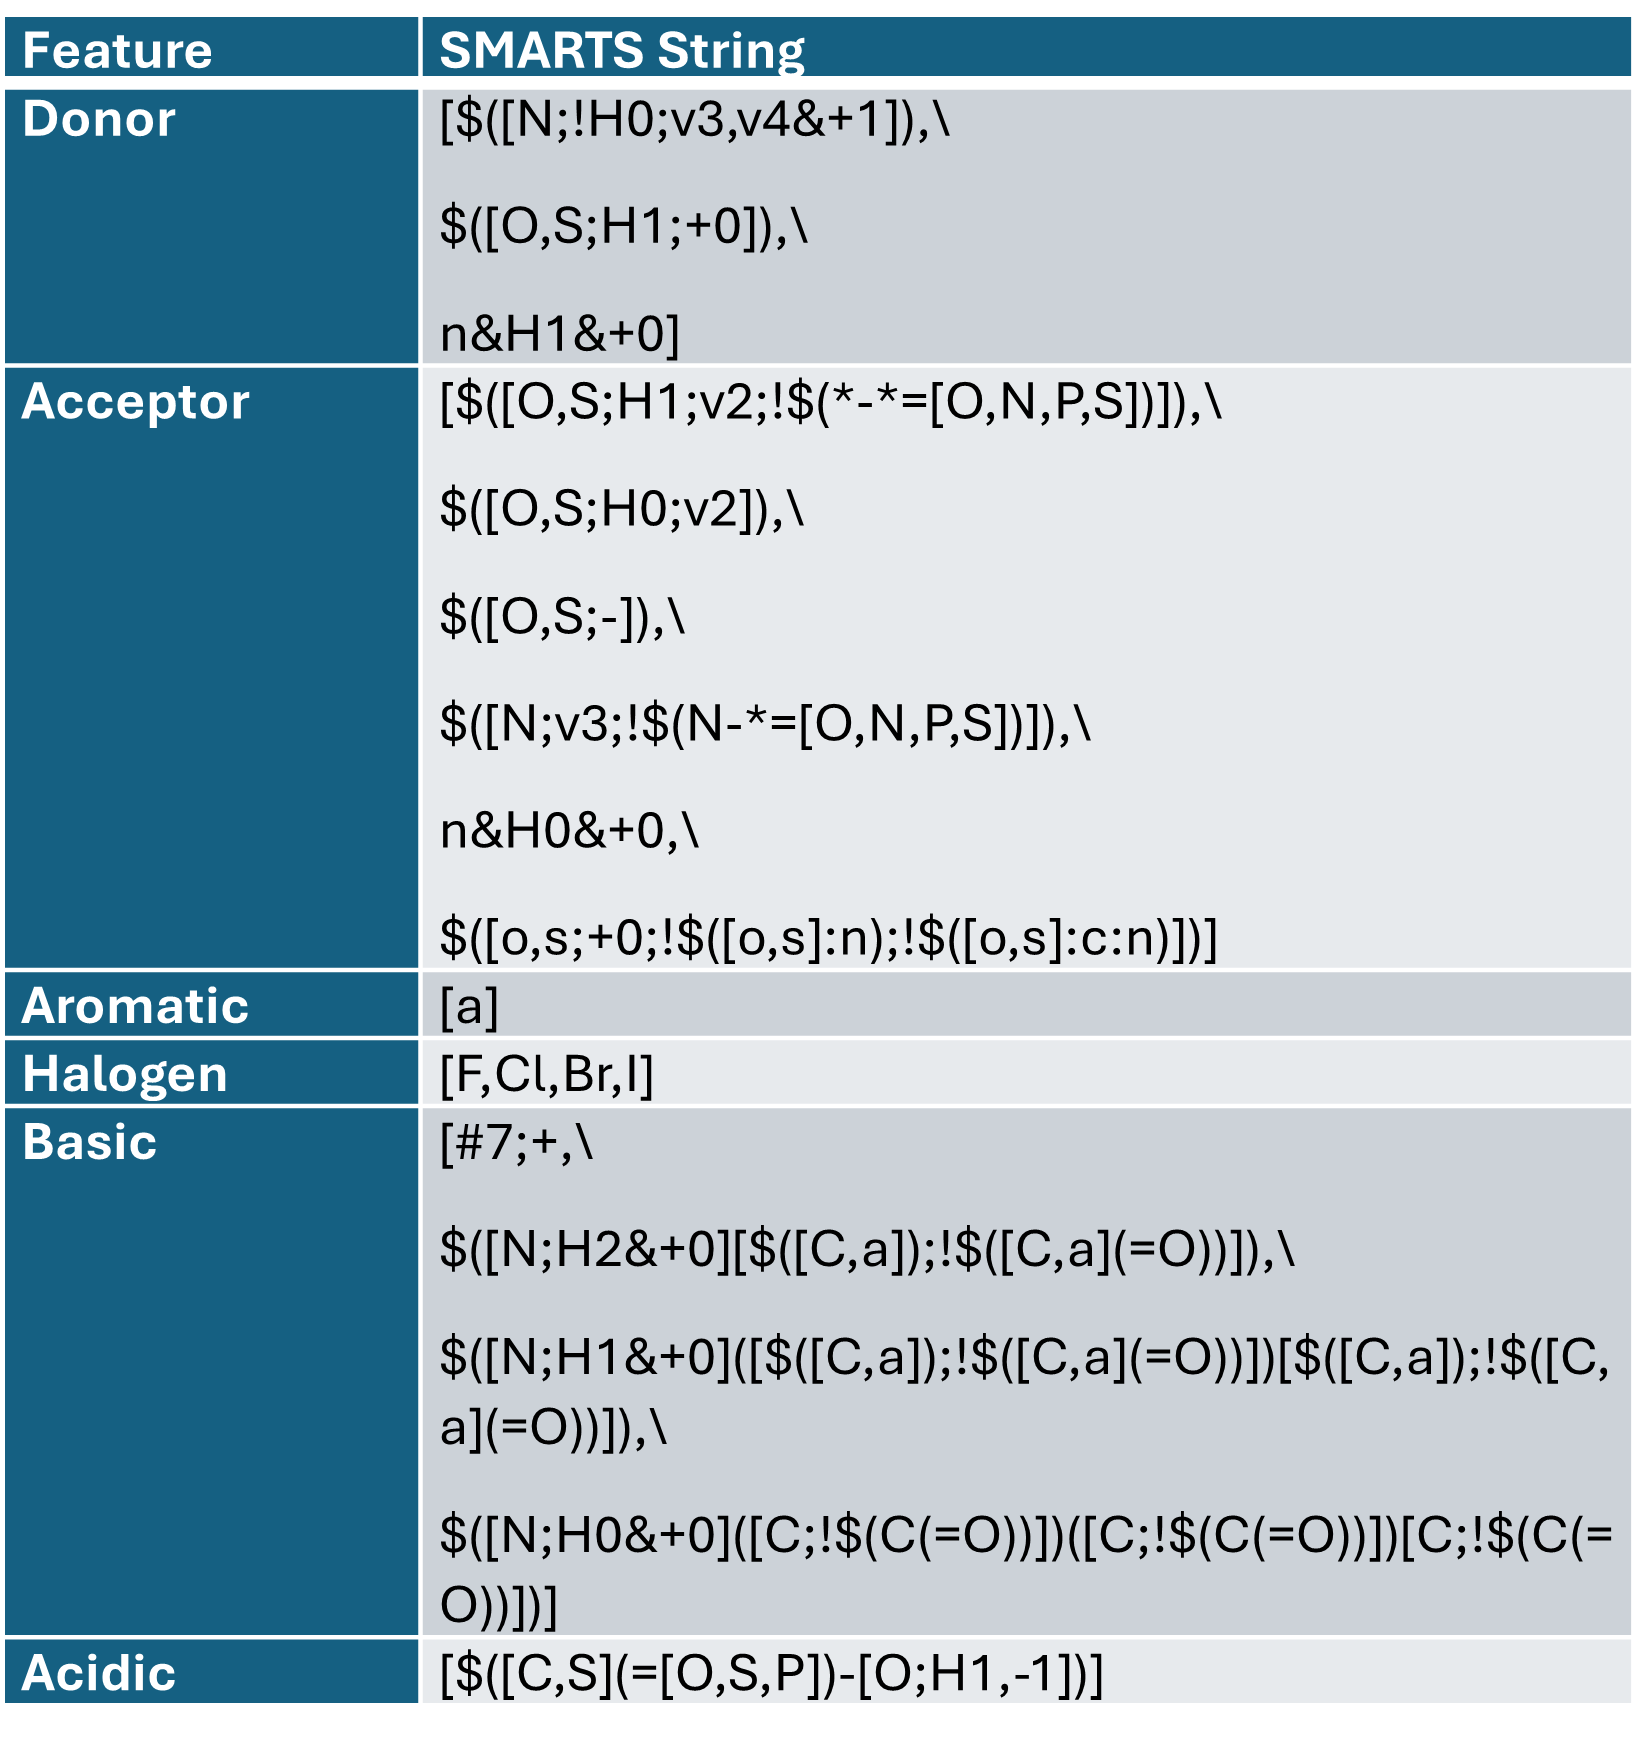
\includegraphics[width=0.8\linewidth]{rdkit_featurefp_features.png}
    \caption{Features used in the Morgan FeatureFP of RdKit}
    \label{tab:rdkit_featurefp_features}
\end{table}

\begin{table}
    \centering
    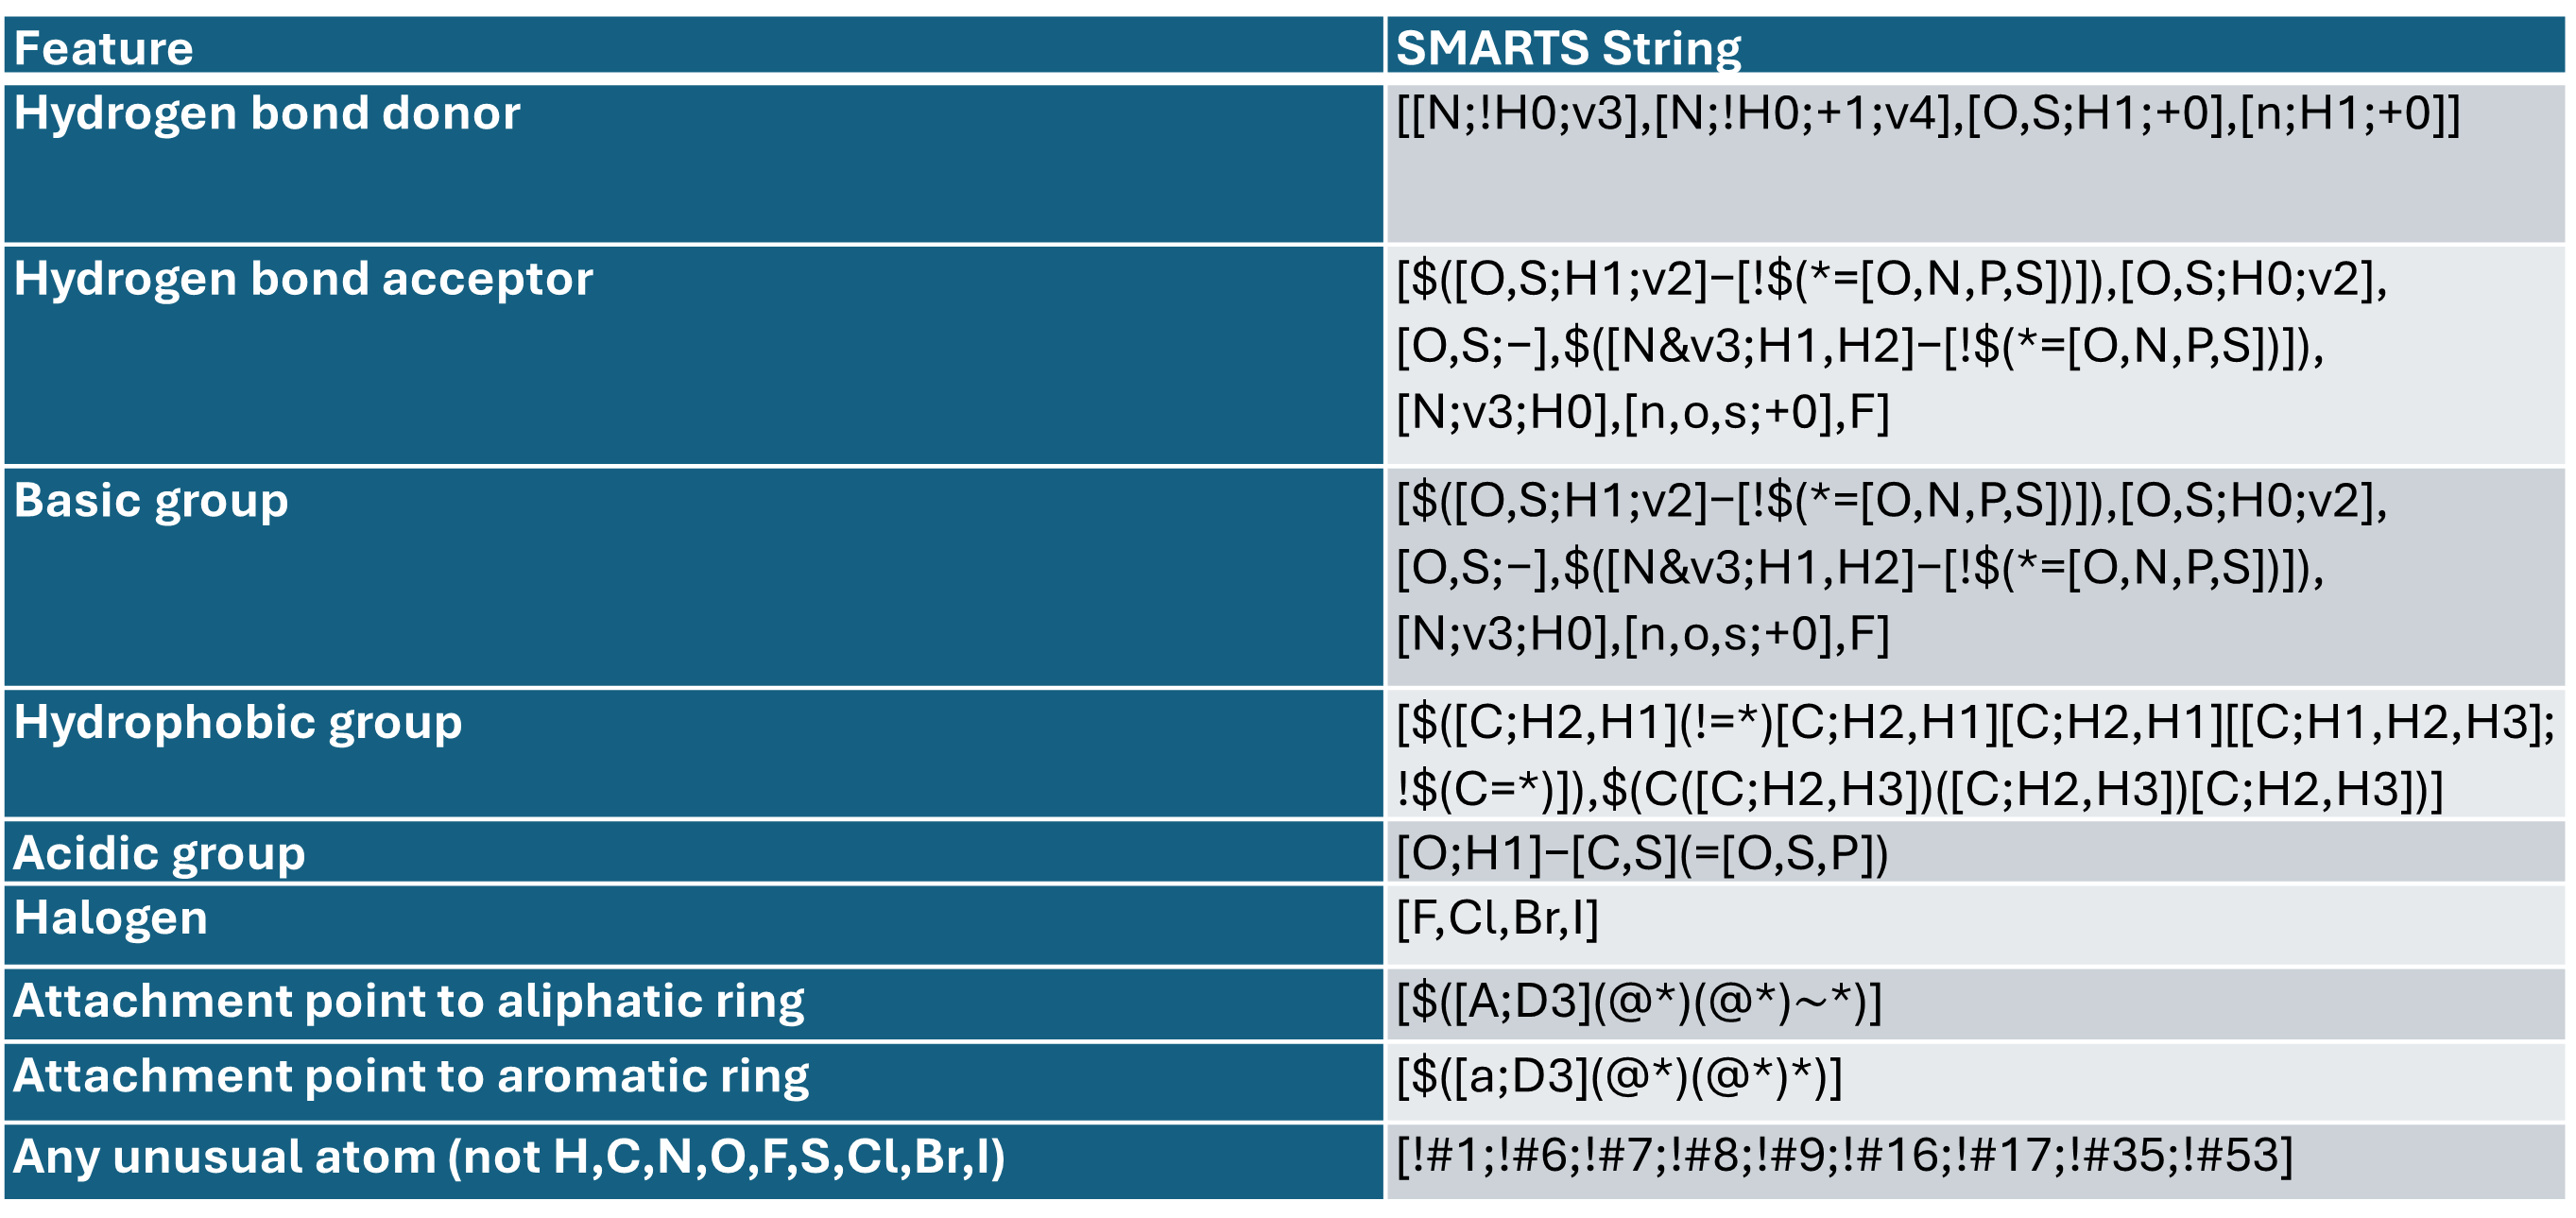
\includegraphics[width=1.05\linewidth]{gobbi_features.png}
    \caption{Features used in Gobbi / Poppinger 1999}
    \label{tab:gobbi_features}
\end{table}



\subsection{Generation of fingerprints}


In addition to the RdKit implementation, also a very simple version of the ECFP fingerprint has been implemented in Python.
This version lacks all the opimizations of the RdKit functions implemented in C, but allows for a very transparent selection of features and different hash functions can be applied.
Furthermore, it allows a custom inclusion of radii, e.g. only the substructures corresponding to the maximum radius, i.e. the more local information can discarded.
Alternatively, custom atom variants can be passed to the RdKit functions.

The feature Morgan fingerprint  uses other features which directly encompass information relevent for biological activity.
Donor, Acceptor, Aromatic, Halogen, Basic, Acidic
The corresponding SMARTS strings are shown in table \ref{tab:rdkit_featurefp_features}.


RdKit also allows to define custom invariants, i.e. one can endow each atom of the molecule with a value; given this value is identical to the values assigned to another atom, the atoms are considered isomorphic.
The effect of this invariants is visualized using 5-Ethyl-2-methylpyridine (\ref{fig:5_ethyl_2_methyl_pyridine}): One time with the full default RdKit feature set (\ref{fig:radius1_all_default_features}), with atomic number only (\ref{fig:radius1_nobonds_onlyatomnr}) , and with topological information only (\ref{fig:radius1_onlytopological}), i.e. all atoms are isomorphic to each other.

\begin{figure}
    \centering
    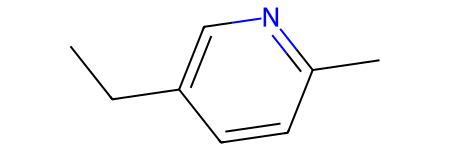
\includegraphics[width=0.75\linewidth]{5_ethyl_2_methyl_pyridine.png}
    \caption{5-ethyl-2-methyl-pyridine}
    \label{fig:5_ethyl_2_methyl_pyridine}
\end{figure}


\begin{figure}
    \centering
    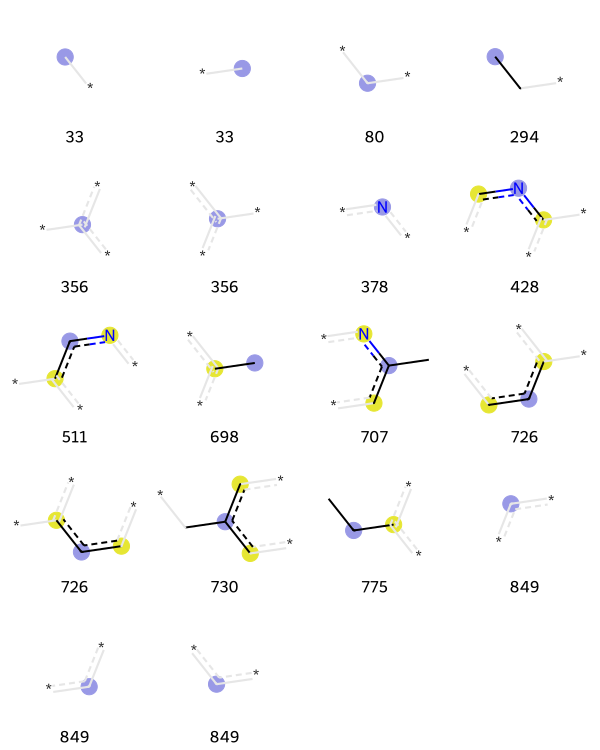
\includegraphics[width=0.75\linewidth]{radius1_all_default_features.png}
    \caption{all substructures up to radius 1; default RdKit features }
    \label{fig:radius1_all_default_features}
\end{figure}

\begin{figure}
    \centering
    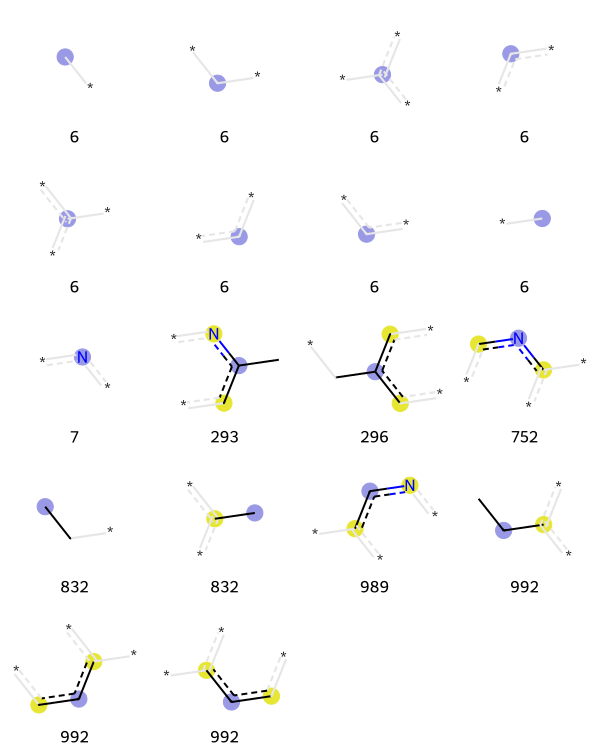
\includegraphics[width=0.75\linewidth]{radius1_nobonds_onlyatomnr.png}
    \caption{all substructures up to radius 1; only atom number as feature, without bond features }
    \label{fig:radius1_nobonds_onlyatomnr}
\end{figure}

\begin{figure}
    \centering
    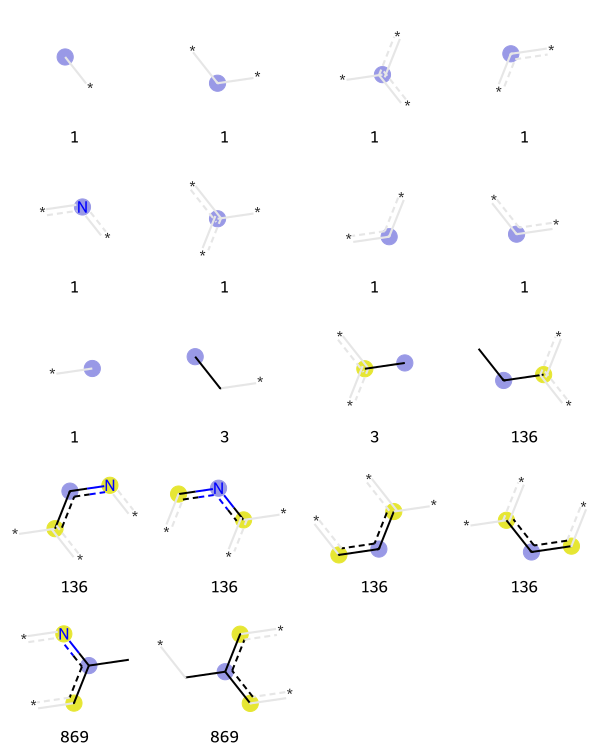
\includegraphics[width=0.75\linewidth]{radius1_onlytopological.png}
    \caption{all substructures up to radius 1; only topological information, without bond features}
    \label{fig:radius1_onlytopological}
\end{figure}

For the protein-ligand interaction task, also the physicochemical fingerprints have been used.





\subsection{Permutation of graph layers}

For assessing the information flow across multiple graph layers, the effect of permutation was studied: After the layer, the output is randomly permuted.

This permutation annihilates the permutation invariance of the graph representation; however, the values and thus statistics like the mean and variance stay the same.

Furthermore, it seems to be plausible that later permutation-invariance annihilating permutations are not that severe because at this stage, all nodes receive information from virtually all other nodes and thus the differences are minor compared to the previous layers. 

\subsection{Important features and (hyper-)parameters}

For obtaining the best hyperparameters for a specific architecture, the Optuna package has been used \cite{Akiba.25.07.2019}.
Hyperparameter optimization posed some peculiar challenges due to the complex nature of the data.
For the GNNS, the main problem is the complex interaction of graph- and classifier-part.
In principle, this could lead to misleading conclusions concerning the performance of the involved graph layers.


\subsubsection{Jumping Knowledge}

Jumping knowledge, as introduced in \cite{Xu.01.10.2018}, allows the combination of the output of the GNN layers in the final aggregation layer.
Different functions for the aggregation have been proposed: Either concatenation of all layer outputs, or the maximum can be used. Alternatively, a LSTM which subsequently processes the layer outputs can be trained.
Jumping knowledge is introduced as means to harness also more intricate, and possibly distant long-range interactions.
In \cite{Xu.01.10.2018}, networks with jumping knowledge performed superior in many tasks. In this context, it is also mentioned that a small number of layers (2) in many tasks performs better than more complex architectures.


Alternatively, one could simply concatenate the output of the individual layers, but apply different activation functions (or other transformation) on the layer-output before it is incorporated into the aggregation.
Given the fact that also ECFPs store the structures found at a smaller radius and do not discard this information, implementation of jumping knowledge or the final concatenation of the layers promises to provide a graph-based representation which is more similar.
For the experiments, also a more sophisticated approach has been implemented, applying on the copied values to be concatenated different operations, e.g. activation functions, than on the values which are processed in the subsequent graph layers (see section 'Custom activation functions').

\subsubsection{Normalization techniques}

Batch Normalization (BN) is a technique used to stabilize and speed up the training of deep neural networks by normalizing the input to each layer. It tackles the internal covariate shift, i.e. a change in the distribution of network activations  due to the change of the distribution of the parameters during training. This phenomenon, called internal covariate shift, makes training harder because the network needs to constantly adapt to these changes.
Batch normalization normalizes the input of each layer by subtracting the batch mean and dividing by the batch standard deviation:

\begin{math}
\hat{x}_i = \frac{x_i - \mu_B}{\sqrt{\sigma_B^2 + \epsilon}}
\end{math},
where $\sigma_B^2$ is the variance and $\mu_B$ the mean of the batch.

Two parameters, $\gamma$ and $\beta$, are learnt for shifting and scaling the normalized output:
\begin{math}
y_i = \gamma \hat{x}_i + \beta
\end{math}
  
On many occasions, batch normalization leads to much faster training. By normalizing the inputs, gradients become more stable, which leads to faster convergence. Furthermore, reduced sensitivity to initialization: The model is less sensitive to the choice of initial weights. Batch normalization also provides regulizarization, it introduces noise because the normalization is based on the batch, which helps prevent overfitting. By doing so, in some cases, it alleviates the need for additional dropout.
        
During inference, BN uses running averages of the mean and variance computed during training.

Layer Normalization (LN) is a similar technique, but instead of normalizing across a batch of examples, it normalizes across the features in a single layer for each data instance individually. This is useful in contexts where batch normalization does not perform well, such as for sequential data or small batch sizes, e.g. it is widely used in Transformers.


\subsubsection{Custom activation functions and binarization of output}

In Duvenaud et al. 2015 \cite{Duvenaud.30.09.2015}, it was stated that the Neural Fingerprint behaves similar to a circular fingerprint for big, random weights.
For an activation function which approximates the binary function, behaviour should therefore become more ECFP-like.

The scaled sigmoid function is defined by:

\[
\sigma_{\alpha}(x) = \frac{1}{1 + e^{-\alpha x}}
\]

and the hardtanh function:

\[
\text{Hardtanh}(x) =
\begin{cases} 
-1 & \text{if } x \leq -1 \\
x & \text{if } -1 < x < 1 \\
1 & \text{if } x \geq 1 
\end{cases}
\]



\begin{figure}
    \centering
    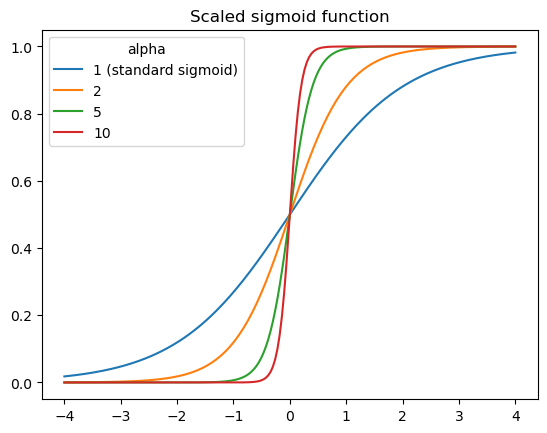
\includegraphics[width=0.5\linewidth]{scaled_sigmoid.png}
    \caption{Enter Caption}
    \label{fig:enter-label}
\end{figure}

In principle, though differentiable, such a steep activation function will lead to training difficulties on many occasions.
Therefore, it is not traced back during backpropagation.
(However, different set-ups would be possible, not only the Straight-Through Estimator.)




\[
\text{ScaledSoftmax}(x_i) = \frac{e^{\alpha x_i}}{\sum_{j=1}^{n} e^{\alpha x_j}}
\]

This allows a combination with the layer concatenation described in the section about Jumping Knowledge.


An alternative approach is the usage of binary neural networks \cite{Yuan.2023} or similar ways to achieve binary output without forgoing differentiability.

A common approach is the Straight-Through Estimator proposed by Hinton in 2012 \cite{Bengio.15.08.2013}. To retain differentiability, during backpropagation the identity function is used instead of the non-differentiable function. This gives (in particular for deep networks) a biased estimate, but was shown to be efficient in practice.



\subsubsection{Pooling and aggregation functions}

\cite{Schweidtmann.2023}

Common aggregation functions are mean, max and sum. For GINs, it has been shown that sum-aggregation has the highest expressivity in distinguishing between input graphs.
(However, it should be stressed again that this does not imply that sum-aggregation always provides the highest performance in specific tasks.)

A more sophisticated choice is Set2Set \cite{Vinyals.19.11.2015}.
This pooling operator is based on a LSTM refinement step.

\begin{align*}
q_t &= \text{LSTM}(q_{t-1}^*) \\
\alpha_{i,t} &= \text{softmax}(x_i \cdot q_t) \\
r_t &= \sum_{i=1}^N \alpha_{i,t} x_i \\
q_t^* &= q_t \, \| \, r_t
\end{align*}

In principle, one can also try to emulate fingerprint-like behaviour by deploying suitable pooling operations.
DiffPool segments the graph into smaller subgraphs using an assignment matrix.
\cite{Ying.22.06.2018}

However, it has to be kept in mind that the fingerprints create subgraphs depending on unique molecular features.

\subsection{Enhanced training strategies}

As outlined in the previous section, activity cliffs as well as the presence of dissimilar molecules in the training set are problematic for the performance of GNNs. Additionally to common methods like dropout and normalization, also a judicious selection of the loss function could improve the results.
For most runs presented, MAE was chosen since this is also mostly used in previous publications on GNNs and molecular property prediction.

Moreover, given the problem of outliers, it seems to be advisable to use a loss function robust in this regard (however, this is two-fold: on the other hand, in some cases, outliers are pair of an activity cliff and it is of great interest to figure out under which circumstances they appear).

In case of Attentive FP, the default parameters of the Pytorch Geometric model have been used.




\subsection{Combination of GNNs and global feature vector}

The potential dependency on global features gives rise to the question how global information could be incorporated into the node representation. On the other hand, perhaps a separation of both steps - i.e. GNN layers and subsequent concatenation with a global ffeature vector - could be even more promising.

In general, numerous variants are possible.
Or implement the global features as attention vector which the nodes can attend to (e.g. via the neural network within the GIN layer).



\subsection{Global feature calculation}

As a further baseline, predictions from global properties alone were computed. 
For the calculation, functions of RdKit were used.


These features include, amongst others, the accessible surface area, the number of specific atoms and the molecular weight (see table \ref{tab:molecular_properties}).

Many of these features are collinear; an appropriate subset has been used.

One could also select all global features indicating the number of occurrences of a particular element. In case that only the number of different atom types is considered, this should be equivalent to a Morgan fingerprint of radius zero and only atom type as invariant.


\begin{table}[h!]
\centering
\begin{tabular}{|l|l|}
\hline
\textbf{Property} & \textbf{Description} \\ \hline
\texttt{molecular\_weight} & The molecular weight of the compound. \\ \hline
\texttt{logP} & The partition coefficient (logP) of the compound. \\ \hline
\texttt{num\_rotatable\_bonds} & The number of rotatable bonds in the molecule. \\ \hline
\texttt{tpsa} & The topological polar surface area of the molecule. \\ \hline
\texttt{num\_h\_donors} & The number of hydrogen bond donors in the molecule. \\ \hline
\texttt{num\_h\_acceptors} & The number of hydrogen bond acceptors in the molecule. \\ \hline
\texttt{molar\_refractivity} & The molar refractivity of the molecule. \\ \hline
\texttt{fraction\_csp3} & Fraction of the molecule's carbons that are sp3-hybridized. \\ \hline
\texttt{num\_heavy\_non\_c\_atoms} & Number of heavy non-carbon atoms in the molecule. \\ \hline
\texttt{num\_carbon\_atoms} & Number of carbon atoms in the molecule. \\ \hline
\texttt{num\_non\_standard\_atoms} & Number of atoms not being C, N, O, or S. \\ \hline
\texttt{num\_nitrogen\_atoms} & Number of nitrogen atoms in the molecule. \\ \hline
\texttt{num\_oxygen\_atoms} & Number of oxygen atoms in the molecule. \\ \hline
\texttt{num\_sulphur\_atoms} & Number of sulphur atoms in the molecule. \\ \hline
\texttt{num\_rings} & Total number of rings in the molecule. \\ \hline
\texttt{num\_atoms\_in\_rings} & Number of atoms that participate in any ring. \\ \hline
\texttt{num\_atoms\_in\_two\_rings} & Number of atoms that participate in two rings. \\ \hline
\texttt{total\_num\_atoms} & Total number of atoms in the molecule. \\ \hline
\texttt{num\_single\_bonds} & Number of single bonds in the molecule. \\ \hline
\texttt{num\_double\_bonds} & Number of double bonds in the molecule. \\ \hline
\texttt{num\_triple\_bonds} & Number of triple bonds in the molecule. \\ \hline
\texttt{num\_aromatic\_bonds} & Number of aromatic bonds in the molecule. \\ \hline
\texttt{total\_num\_bonds} & Total number of bonds in the molecule. \\ \hline
\end{tabular}
\caption{Description of global molecular properties.}
\label{tab:molecular_properties}
\end{table}



\section{Differences between Graph Neural Network-based representations and Morgan fingerprints}

Again, the question whether different molecular graphs are distinguishable for a specific architecture has to be separated from the performance on a learning task.
However, the differences are a little bit more nuanced: 
At first glance, the number of layers of a (standard, i.e. non-higher order) GNN architecture resembling the radius of the Morgan Fingerprint: In the first layer, information of the neighbours is incorporated into the feature vector of each node; at the next layer, the neighbours of a specific node already contain information about the neighbours of the neighbours of this node and so information of nodes which are two edges far away is incorporated, etc.

Indeed, for radius 1, the unique entries are, as expected, identical.


The workflow of the Morgan Fingerprint suggests the processing of subgraphs: In the first iteration of the Morgan algorithm, all rooted subgraphs of radius 1 are investigated, at the next iteration of radius 2, and so on. 
A construction of all rooted subgraphs of a specific size of the molecular graph and subsequent counting of isomorphic subgraphs should give the same result as the Morgan Fingerprint (but is, due to the complexity of determining isomorphic subgraphs, computationally much more demanding), exempt for events like hash collisions.

In particular, the results in this study (presented in the next section) as well as in previous publications also show that GIN architectures do not perform equal to Morgan Fingerprints (usually, the effect of frozen layers is not investigated; however, one would not assume that freezing fully removes the differences, in particular in those cases in which GINs perform worse).

A straightforward approach for creating a neural version of a Morgan Fingerprint would thus create all subgraphs up to a given radius and then perform usual GNN operations on these subgraphs.

Nested Graphs should give a similar number of subgraphs.


For the determination of isomorphic subgraphs, the Weisfeiler-Leman algorithm as well as an exact algorithm were applied (for both, the NetworkX-library was used).

	\chapter{Results}

The evaluation of performance differences is of utmost importance since it also influences the reliability of claims that refined architectures like the Attentive Fingerprint are capable of learning generalizable knowledge about molecular structures (and, because such knowledge is crucial for accurate predictions, outperform previous models).

Similarly, it could be insightful to check whether the same difference ranking occurs for different runs and, in case of different splits, and whether similar molecules – or the same molecules in case they appear multiple times in the test set – behave also similarly.

A thorough comparison of all these schemes is beyond the scope of this work.
In some cases, probably optimal solutions are thus overlooked and one should generalize with caution.

The focus was rather on two related questions:

\begin{enumerate}
	\item Which factors can help explain the differing results in previous work?
	\item Are there at least some basic guidelines for deciding which method is better performing?
\end{enumerate}

This issue is very common, compare e.g. the results in \cite{Jiang.2024,Liu.2025}.

\subsection{Preliminary remarks}

If the main reason for an inferior performance of GNNs compared to Morgan Fingerprints is overfitting, whereas the ability to discern substructures is equal, it should be possible to compensate for these detrimental factors by techniques like dropout or altered training data and achieve at least equal performance.

It should be further stressed that the differences in performance presented are usually rather small.
In this regard, it is also a central goal to assess which architectural decisions really matter.

After a first investigation, it turned out that the datasets differ highly in difficulty: Whereas for some (e.g. the ESOL dataset), all architectures achieve 'good' results, for other ones even a positive correlation between true and predicted values is hard to achieve; in some cases, suboptimal parameters lead to horizontal curves for regression tasks.


In particular, one should also point at the danger of biases in the datasets itself.

In principle, it could be that the GCN architecture produces the same output for different molecules. However, with respect to the training task, this can be appropriate (for a binary classification task, it would suffice to map all molecules to exactly two numbers etc.)


Therefore, in cases for which a modified architecture was used, but hyperparameter optimization was not done anew, one should be aware that in principle a further improvement could be possible. (This is in particular true for extended, more complicated architectures, like the combining of layers.)


Analogously, for classification tasks, one has to check whether the ratio between the classes affects molecular fingerprints differently than graph representations.


(Most of the datasets were used in other studies evaluating either the performance of Morgan fingerprints or graph representations; however, due to the problems elaborated on above, a comparison was impossible.)

A major incentive for the application of very diverse datasets was the detection of differences in performance.


The main goal was to get a rough overview of whether or what differences and size there are between the architectures.

In some cases, default values are omitted for a clearer representation (e.g., the default for Jumping Knowledge is ‘None’, equally for dropout and normalization layers, and also usually no frozen layers are applied).

\section{Comparison of embeddings and substructures on 'toy examples'}

In principle, it should therefore be possible to replicate the feature vector generated by the Morgan algorithm by using GNNs. 

Again, it has to be stressed that the maximizing of expressivity, i.e. the ability to distinguish between input graphs, is not a conditio sine qua non for success in the molecular property prediction tasks. In fact, it can be a hindrance; in particular for binary classification tasks, a mapping onto two different feature vectors would be sufficient.

One possibility is to ‘train’ the network with all weights frozen.
Comparison with the trained version shows whether trained parameters lead to a diminished differentiation of graphs (which is not necessarily accompanied by a drop in performance, but can even be beneficial).

(For reasons of efficiency, it cannot be recommended to use such a neural network in practice; in almost every scenario, the computation of the fingerprints is much faster and less resource-intensive than the instantiation – or even training, which in case of frozen layers can be partly ignored – of a neural network.)


RdKit also supports the computation of rooted fingerprints: Instead of one fingerprint for the full molecule, for specific atoms all substructures are outputted (in case of the Morgan fingerprint, this means all substructures of the specified radius with the selected atom as central atom).

Summing up of all rooted substructures should yield a fingerprint equivalent to the molecule fingerprint; however, there will be substructures counted multiple times.


number of unique nodes per embedding

\section{Hyperparameter optimization}

If not stated otherwise, in the boxplots all information given before 'opt. hyperparameters' indicates fixed parameters (this is important since parameters to be optimized in some runs are treated as fixed in other ones, e.g. Jumping Knowledge).

\section{Inter- and intra-run variance}

To illustrate this problem, for the ESOL dataset the variances for ten runs on the same split (i.e. only the random seed changes, train and test data are identical), and on ten different splits for the optimized parameters are shown.
To disentangle variance between runs on the same data and variance due to different splits, 10 runs of the same architecture with the same data were performed (so only the random seed has changed).
As one sees, even for the same data differences between runs are considerable.


\section{Results for specific datasets / General outcome}

For most datasets, a radius of 2 in combination with a fingerprint size of 2048 performs best. This is in line with the results in \cite{Deng.2023} and \cite{Stepisnik.2021}. Similarly, for GNNs, more than one or two layers usually do not provide optimal results.
(For GINs, the activation function makes a huge difference.)

Only for datasets / splits which are very difficult (partly giving rise to performance hardly better than a random classifier), higher radii or layer numbers are selected by hyperparameter optimization.

It must be noted that due to the classification layer the evaluation becomes much more complex:
In particular, there are optimal combinations with a rather complex, expressive graph architecture and a thin final classifier as well as such ones with a small graph part and a final classifier consisting of multiple dense layers consisting of many neurons.


In the setting with one layer of the same size as the graph output channels, dropout has rather high (e.g. 0.15, in same cases 0.5) values. Usually, a more compact classification layer is used.

\subsection{ESOL}

\begin{figure}
    \centering
    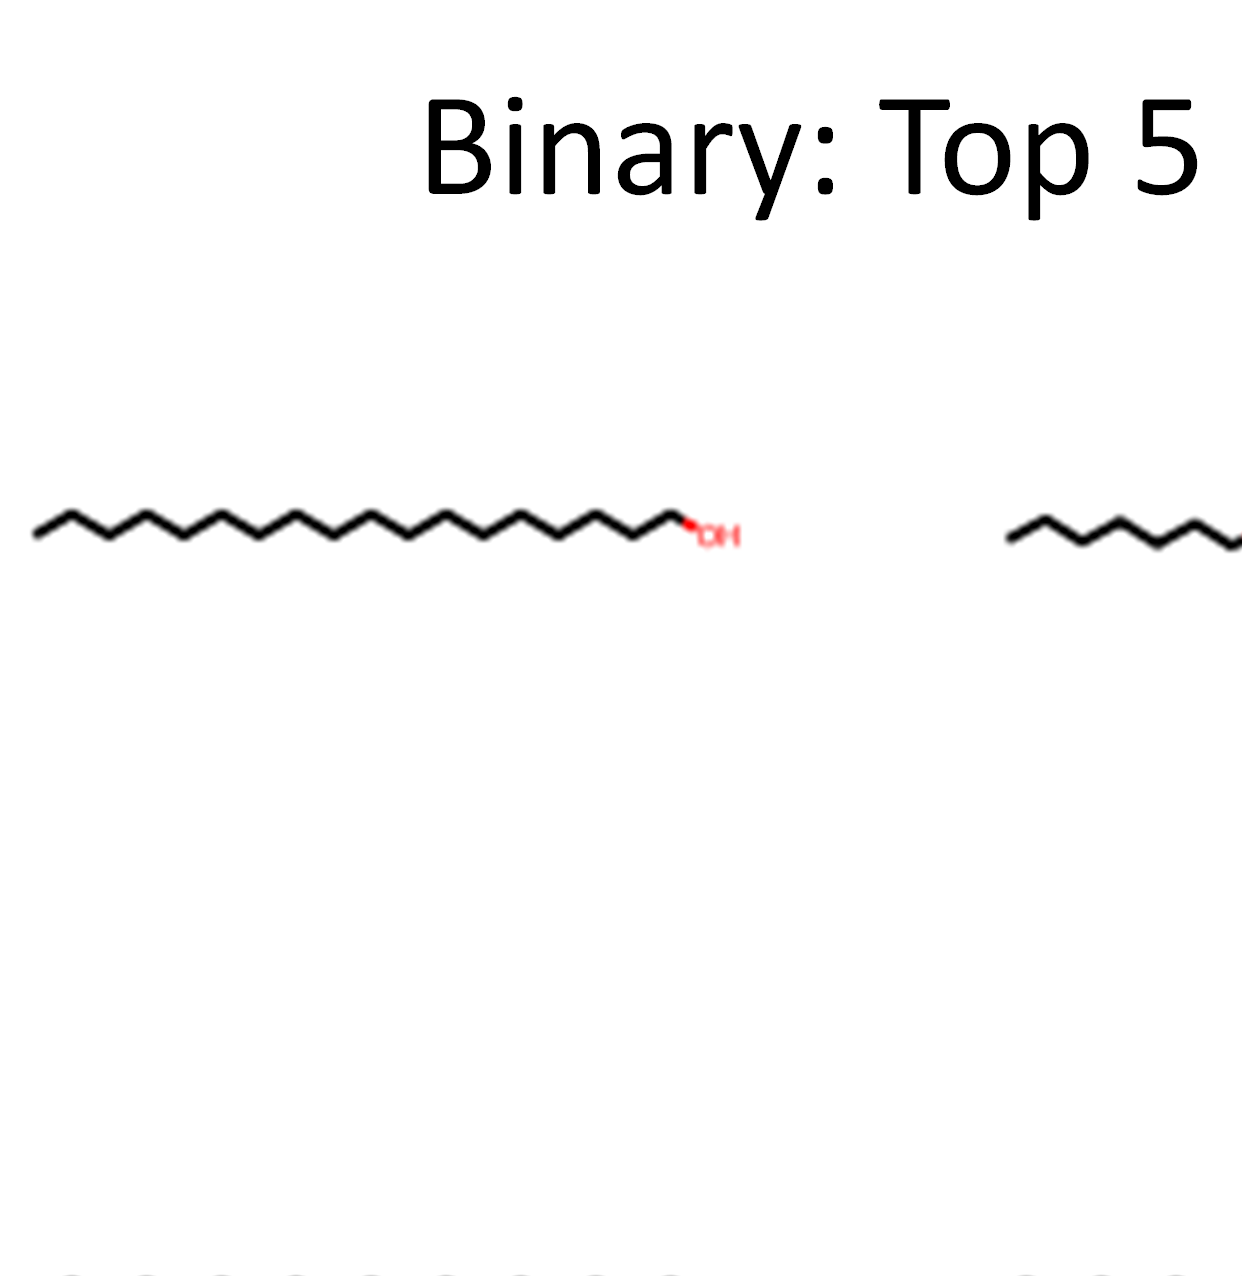
\includegraphics[width=0.25\linewidth]{binary_count_similarity_esol.png}
    \caption{Molecules with top simliarity / ESOL dataset}
    \label{fig:binary_count_similarity_esol}
\end{figure}


\begin{figure}
    \centering
    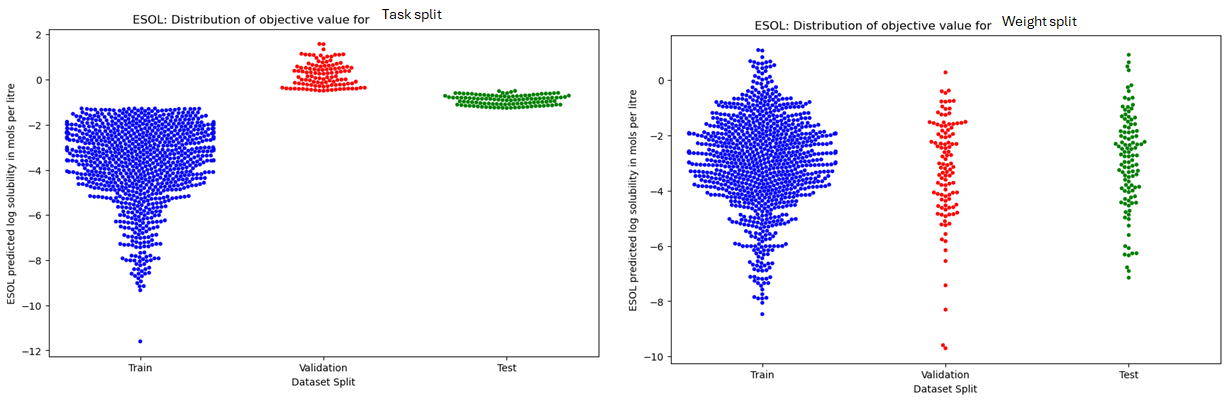
\includegraphics[width=1.15\linewidth]{weight_task_esol.png}
    \caption{Distribution for Task and Weight split on the ESOL dataset}
    \label{fig:weight_task_esol}
\end{figure}


These differences on the task split call for further explanations.



\begin{figure}
	\centering
	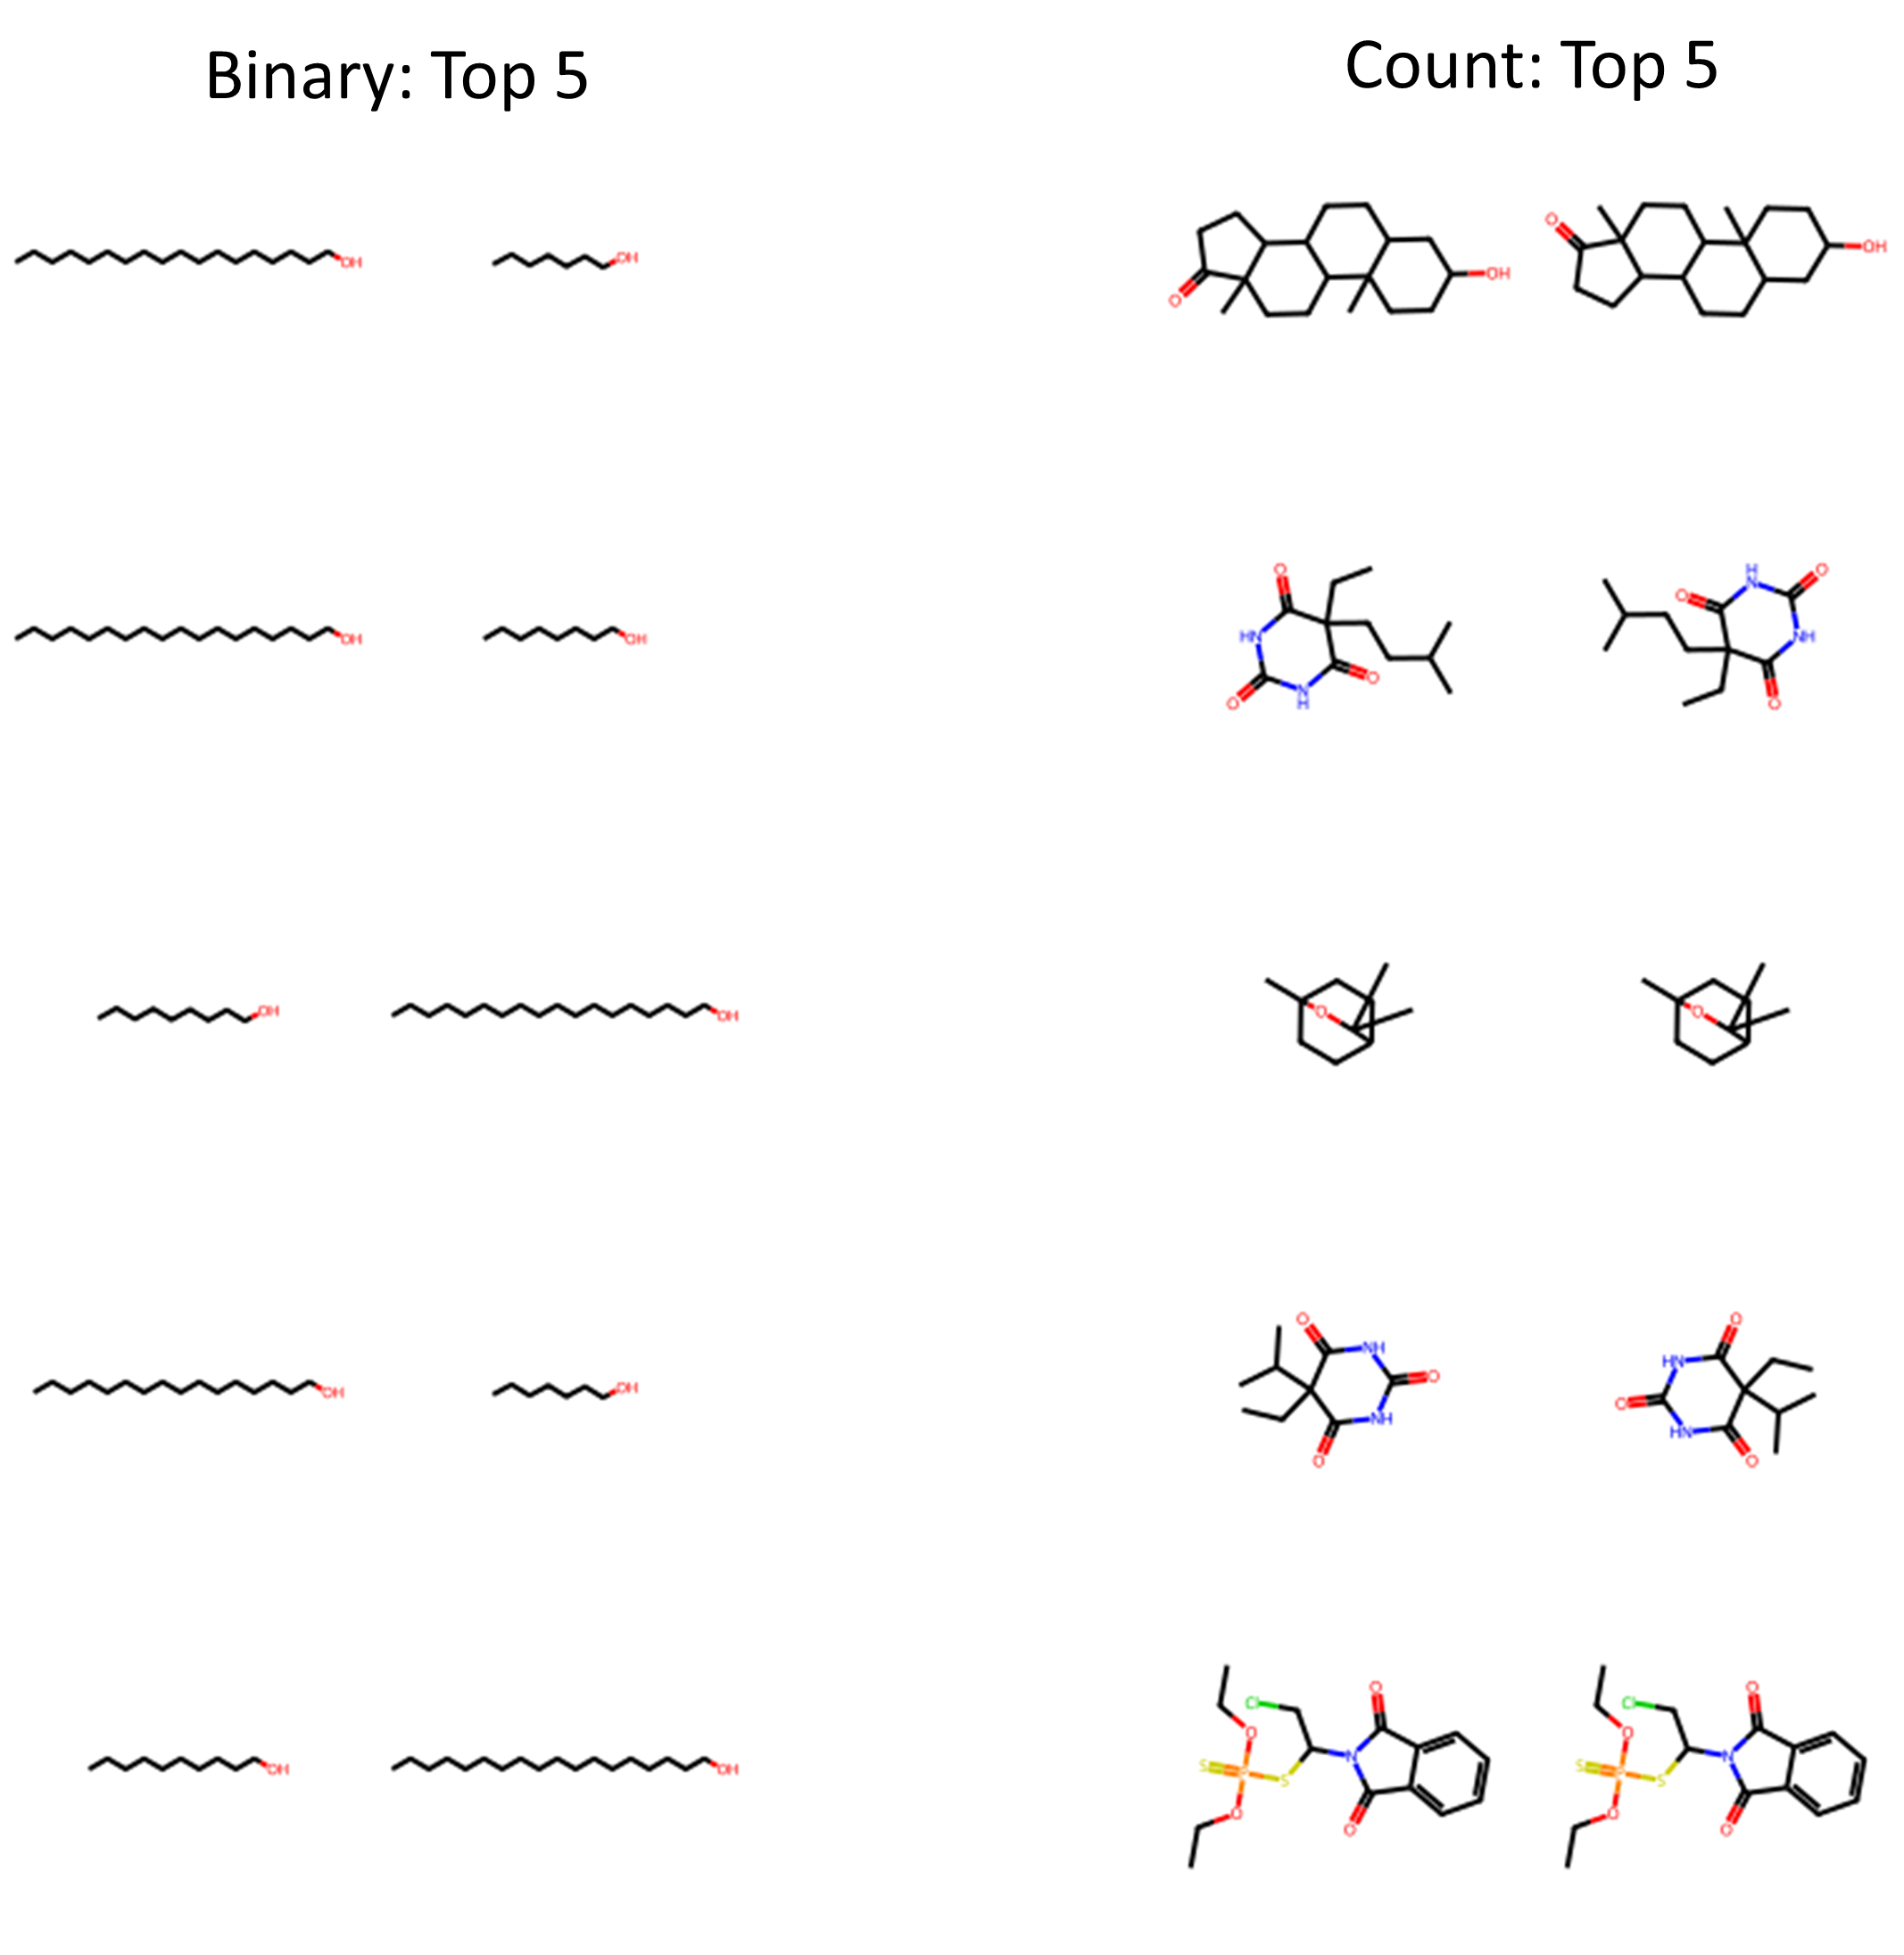
\includegraphics[width=1.15\linewidth]{esol_top5_similarity_binary_count.png}
	\caption{esol_top5_similarity_binary_count}
	\label{fig:esol_top5_similarity_binary_count}
\end{figure}

\ref{fig:esol_top5_similarity_binary_count} clearly shows this effect.


\subsection{BACE}

On this classification task, for many splits classical fingerprints combined with a dense layer perform better than GIN or GCN models.

\subsection{Lipophilicity}

Similarly to the ESOL dataset, an impaired performance of binary Morgan fingerprints in comparison to count-based versions is discernible on the Lipophilicity dataset trained with L1 loss function; however, the difference is rather small.
Interestingly, GINs show a significantly smaller L1 error.
The investigation of the variance shows an even more pronounced difference between Morgan fingerprints and GINs.

\begin{figure}
    \centering
    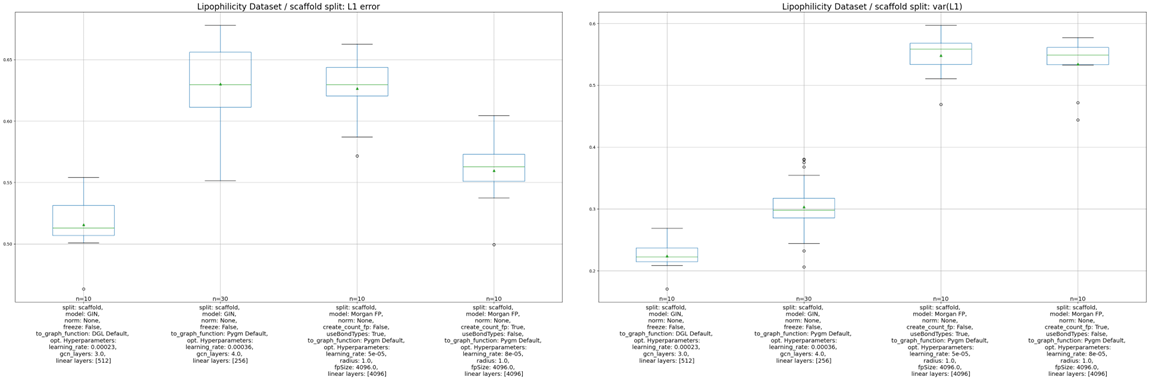
\includegraphics[width=1.00\linewidth]{lipophilicity_res1.png}
    \caption{Lipophilicity dataset: Mean and variance of L1 error}
    \label{fig:lipophilicity_res1}
\end{figure}

Lipophilicity on Task Set!

\subsection{Size and classifiers on the ZINC dataset}


\begin{landscape}
    \centering
    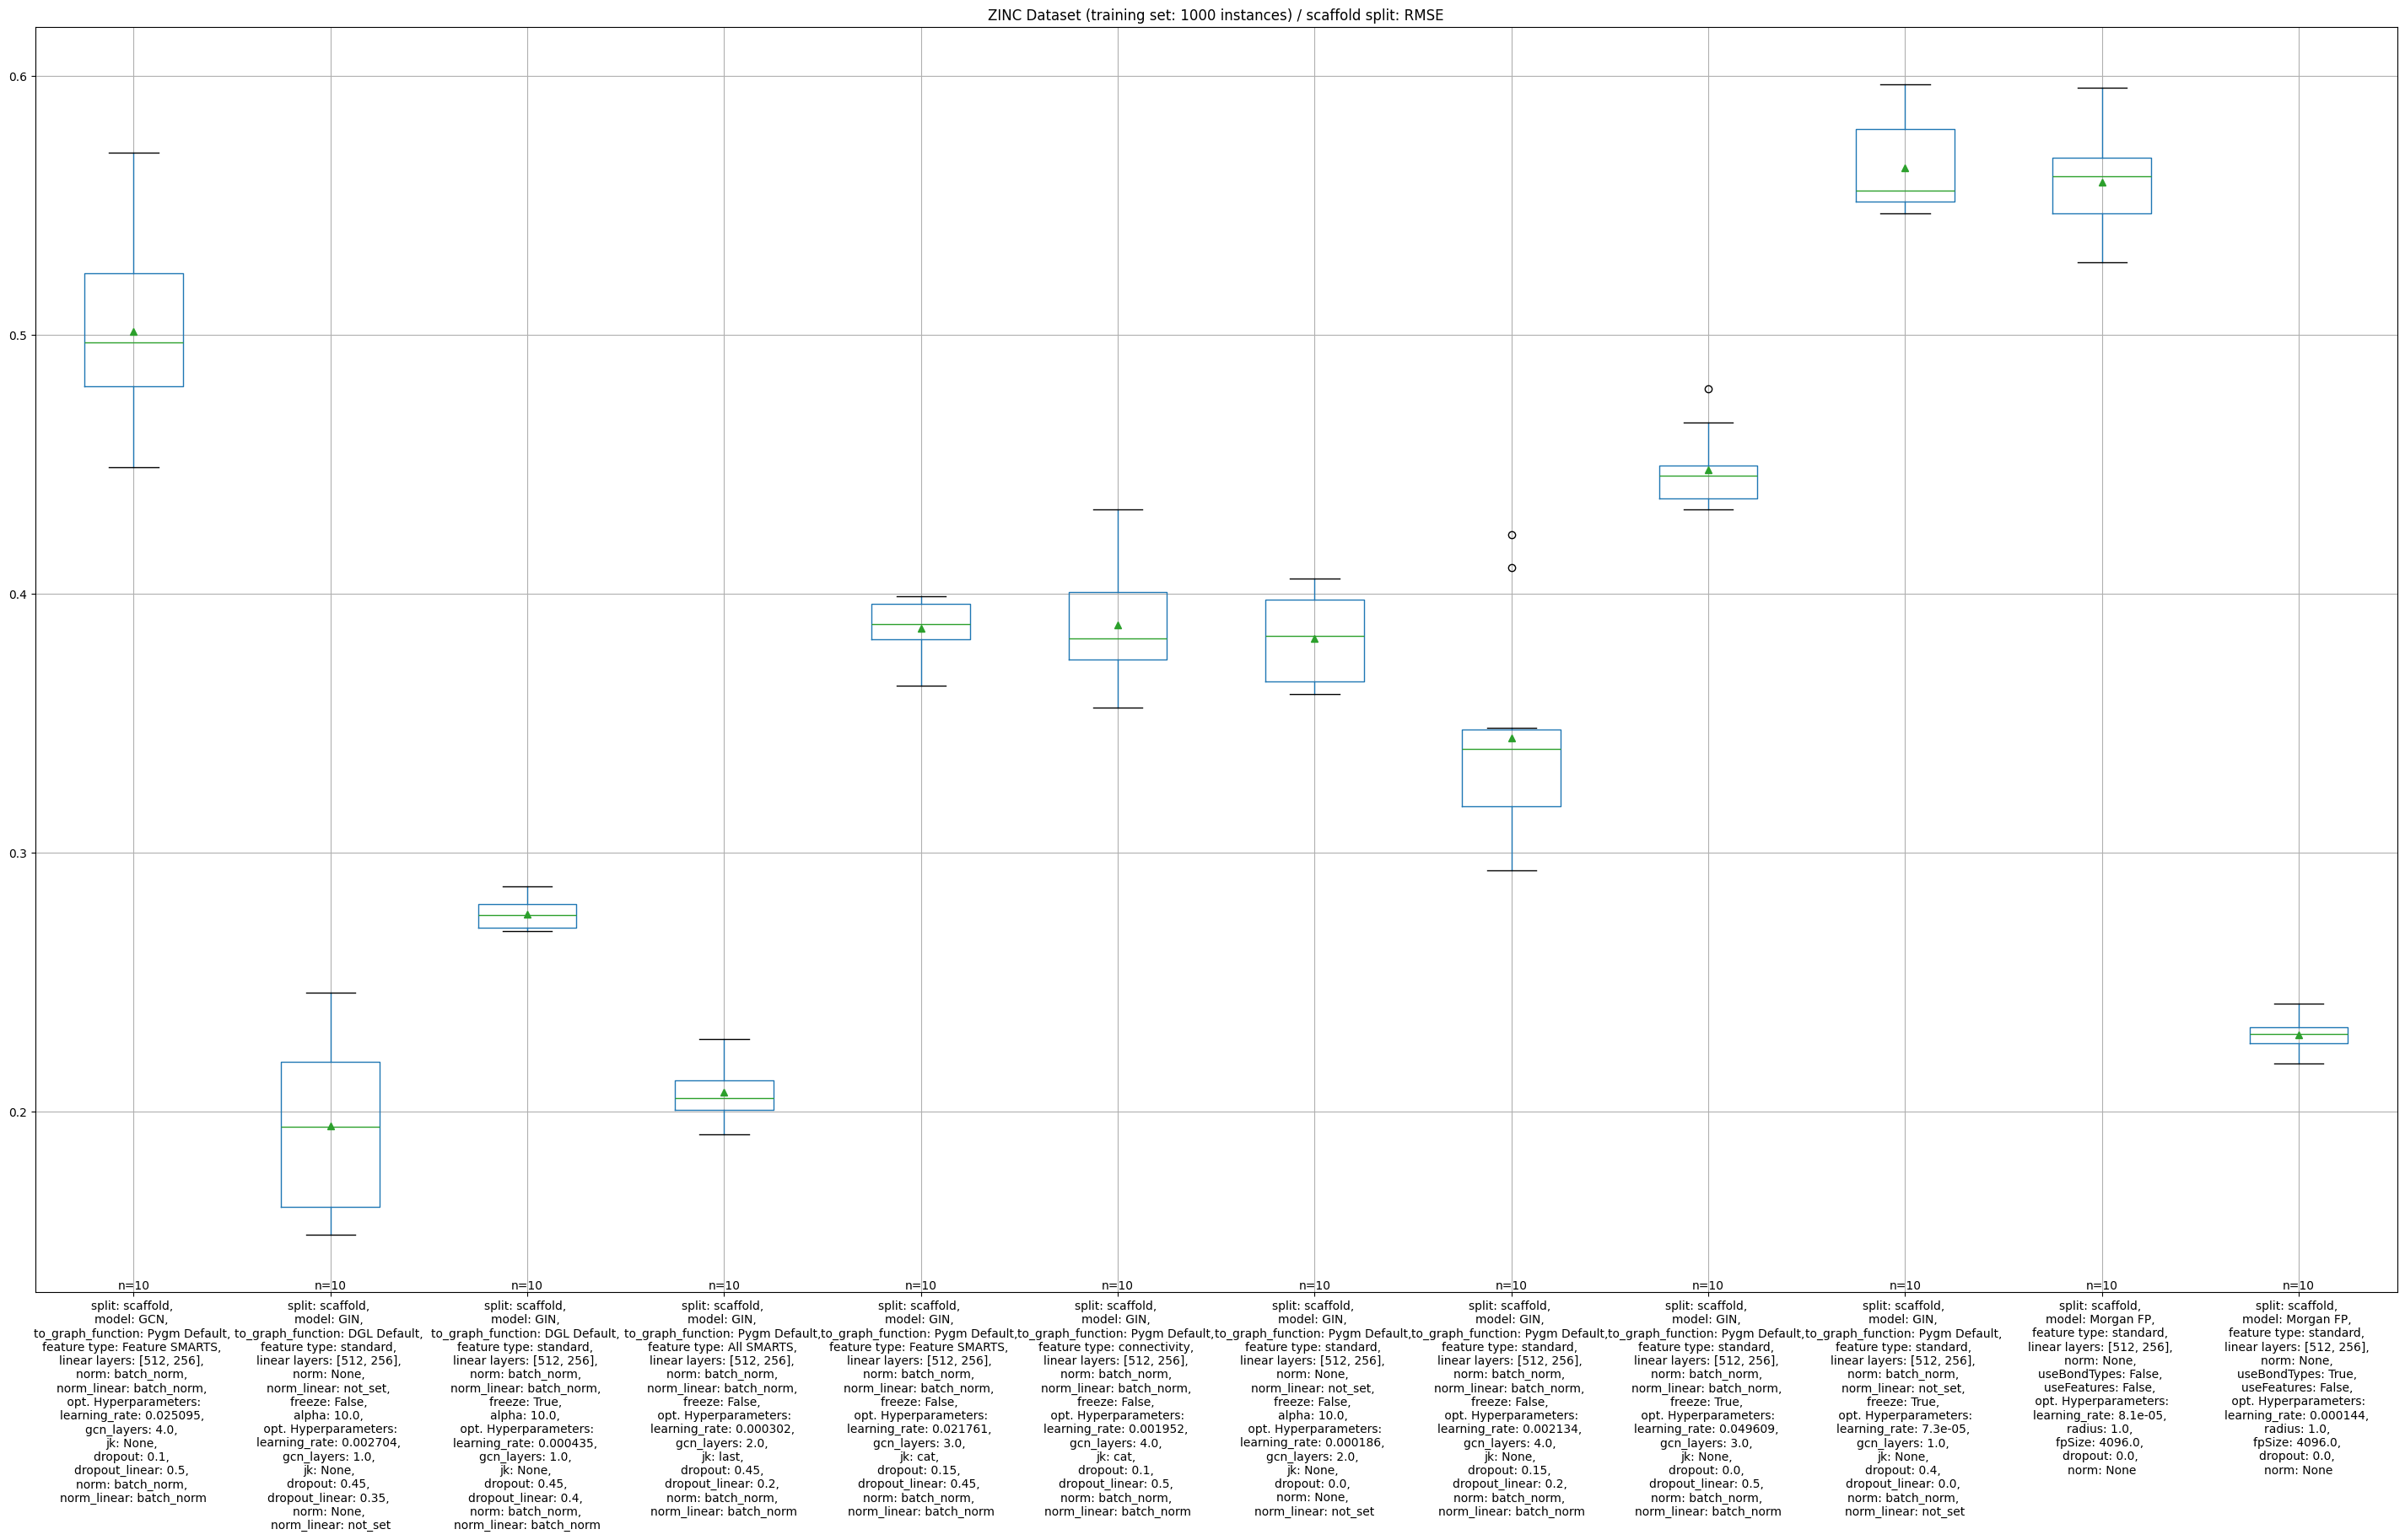
\includegraphics[width=1.05\linewidth]{zinc_1000_scaffold_all1.png}
    \caption{Results for ZINC (1000 training instances) hyperparameter optimization}
    \label{fig:enter-label}
\end{landscape}

Again, frozen parameters with batch normalization perform far worse. Thus a more detailed comparison between such runs with and without batch normalization is advisable.

Interestingly, in this case the Scaled Sigmoid activation function with a high alpha (inducing almost step-function like behaviour) performs best.



It is also one of the rare occasions in which one GNN architecture (GCN) apparently performs much worse than another one (GIN); however, it would be necessary to check this for different feature set configurations.




The enormous size of the ZINC dataset allows for a systematic investigation.
For the ZINC dataset, one could, e.g., use subsets of
500, 1000, 5000, 10000 and 20000 data instances in the training set.

However, linear regression provides almost equally good results.


\subsection{LIT-PCBA dataset}

The LIT-PCBA dataset poses extraordinary challenges due to class imbalance and the creation of the split (see methods).


For this dataset, also an additional run was done.

\subsection{Activity Sets}

The Dopamine dataset is extremely small.

For HERG, much more data is given, leading to a much longer training time.


\section{Influence of the final classifier layer}

In particular, since previous results have shown that this relation is complex, the impact of the final classifier layer has been studied: A richer, more expressive graph representation possibly performs better with a more compact classifier, whereas a small graph readout perhaps needs a bigger (in terms of the number of layers as well as the number of neurons per layer) MLP to extract meaningful features.





Hyperparameter optimization and the set up of the models aimed at maximal flexibility and full control over all parameters. For instance, the values for dropout and batch norm can be applied independently for the GNN part and the subsequent classifier


Interestingly, even with batch norm usually considerably high dropout values (for the graph layers as well as for the dense classifier) are chosen.

In principle, the learnable parameters should not change the ability to discern between molecules and substructures, but the task.
This also implies that a very shallow, simple final classifier leads to greater differences between frozen and learnable parameters.



\section{Splitting-related effects on performance}

In line with expectations, errors are in particular high for values at the margins of the distribution.

For selected datasets, the effect of splitting was investigated.

It should be noted that in previous analyses this was usually not done: Random and scaffold splits were mostly performed, but it was not checked how these split techniques effectively alter the data sets and whether they indirectly cause a task split, i.e. a split concerning the distribution of the objective value.

Fig. \ref{fig:weight_split_esol} and \ref{fig:weight_split_esol_var_mse} show results for 30 runs on the same weight split (so again intra-run variance is measured).
One sees that the variance (although only the random seed has changed) are even much more pronounced than for the random split.

\begin{figure}
    \centering
    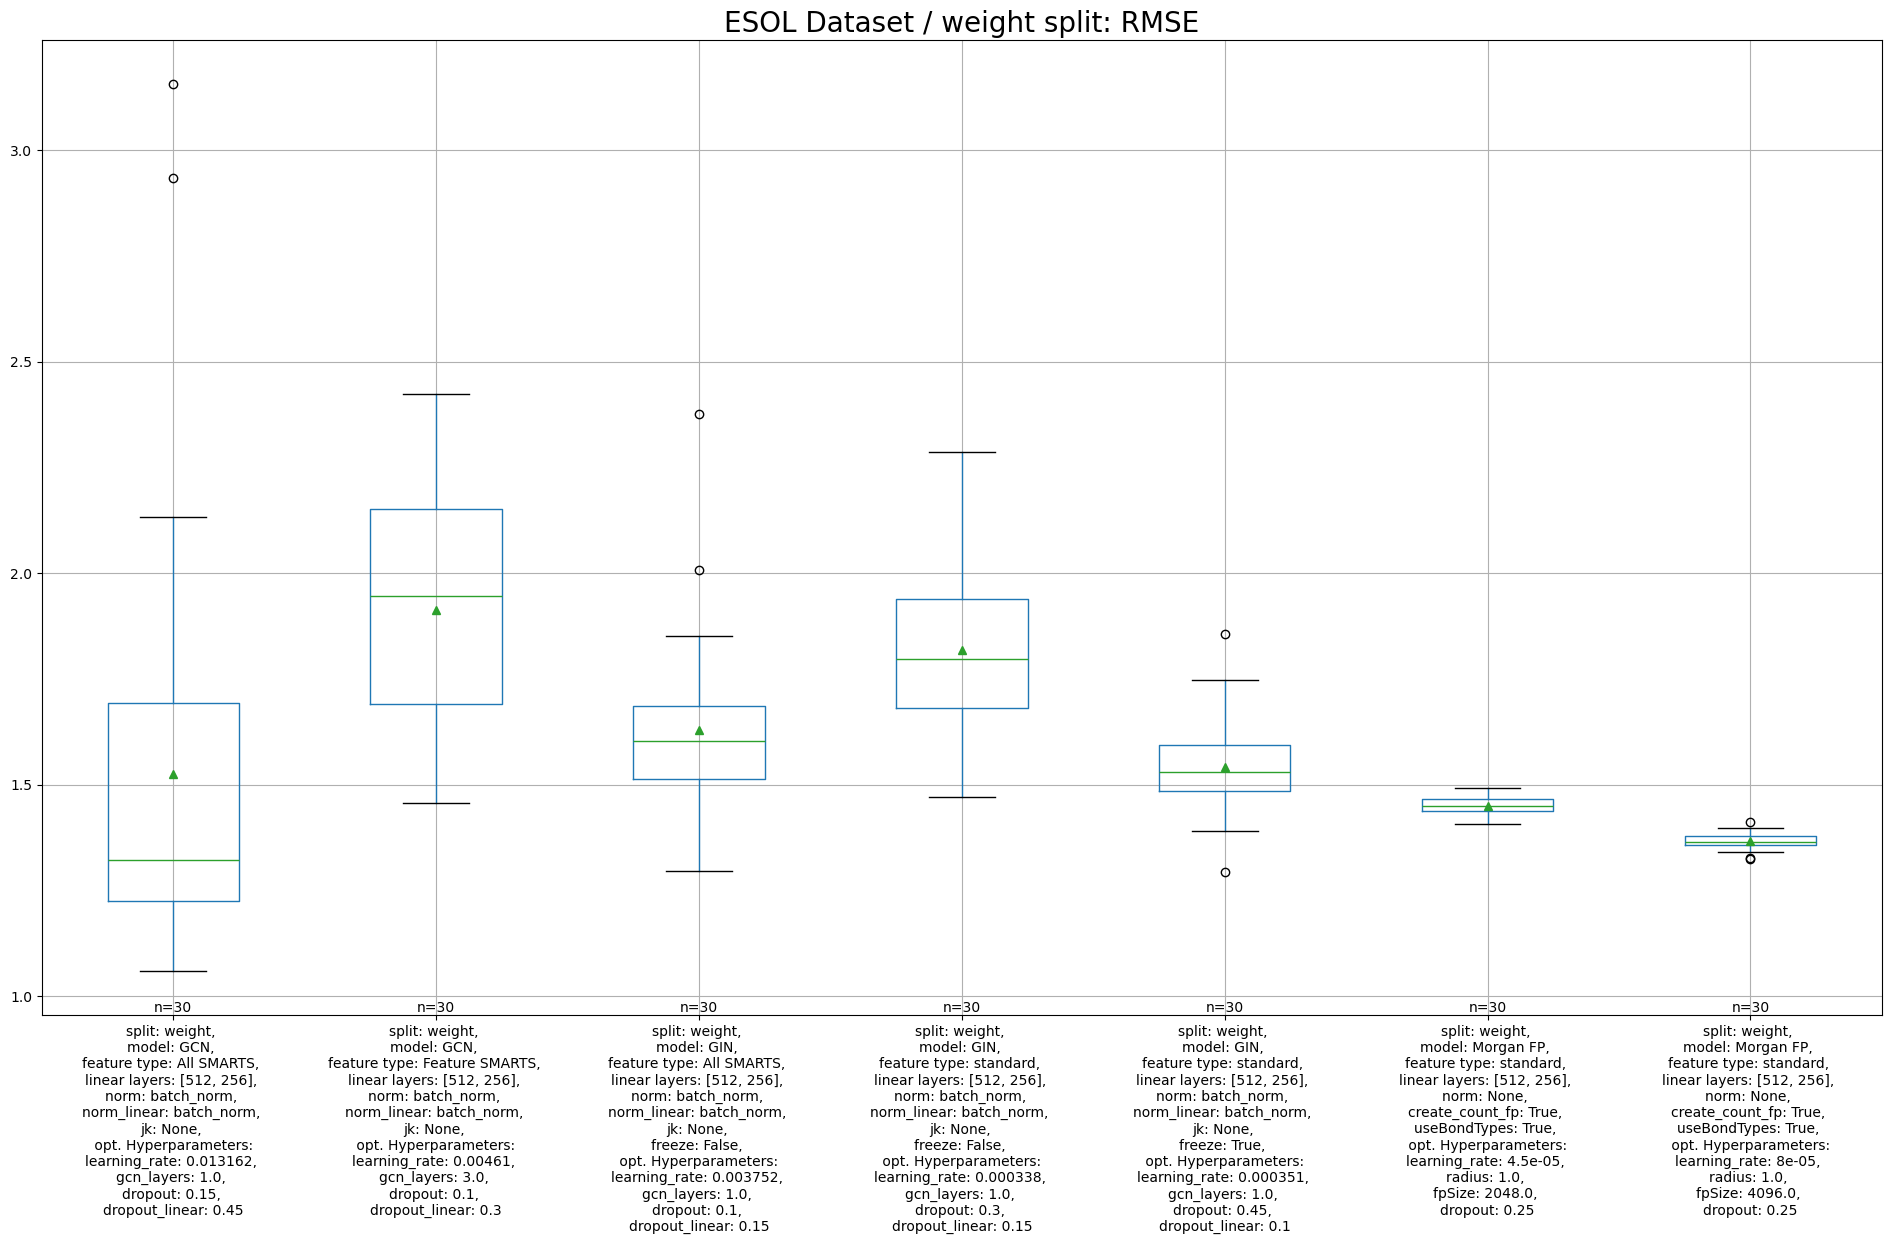
\includegraphics[width=1\linewidth]{weight_split_esol.png}
    \caption{Boxplot three and four as well as five and six show two independent runs with hyperoptimization. The differences in terms of performance as well as found hyperparameters highlight the problems outlined above again. However, the optimized parameters are nonetheless very similar for all architectures; one (or max. two) GNN layers seem to be optimal.}
    \label{fig:weight_split_esol}
\end{figure}



\begin{figure}
    \centering
    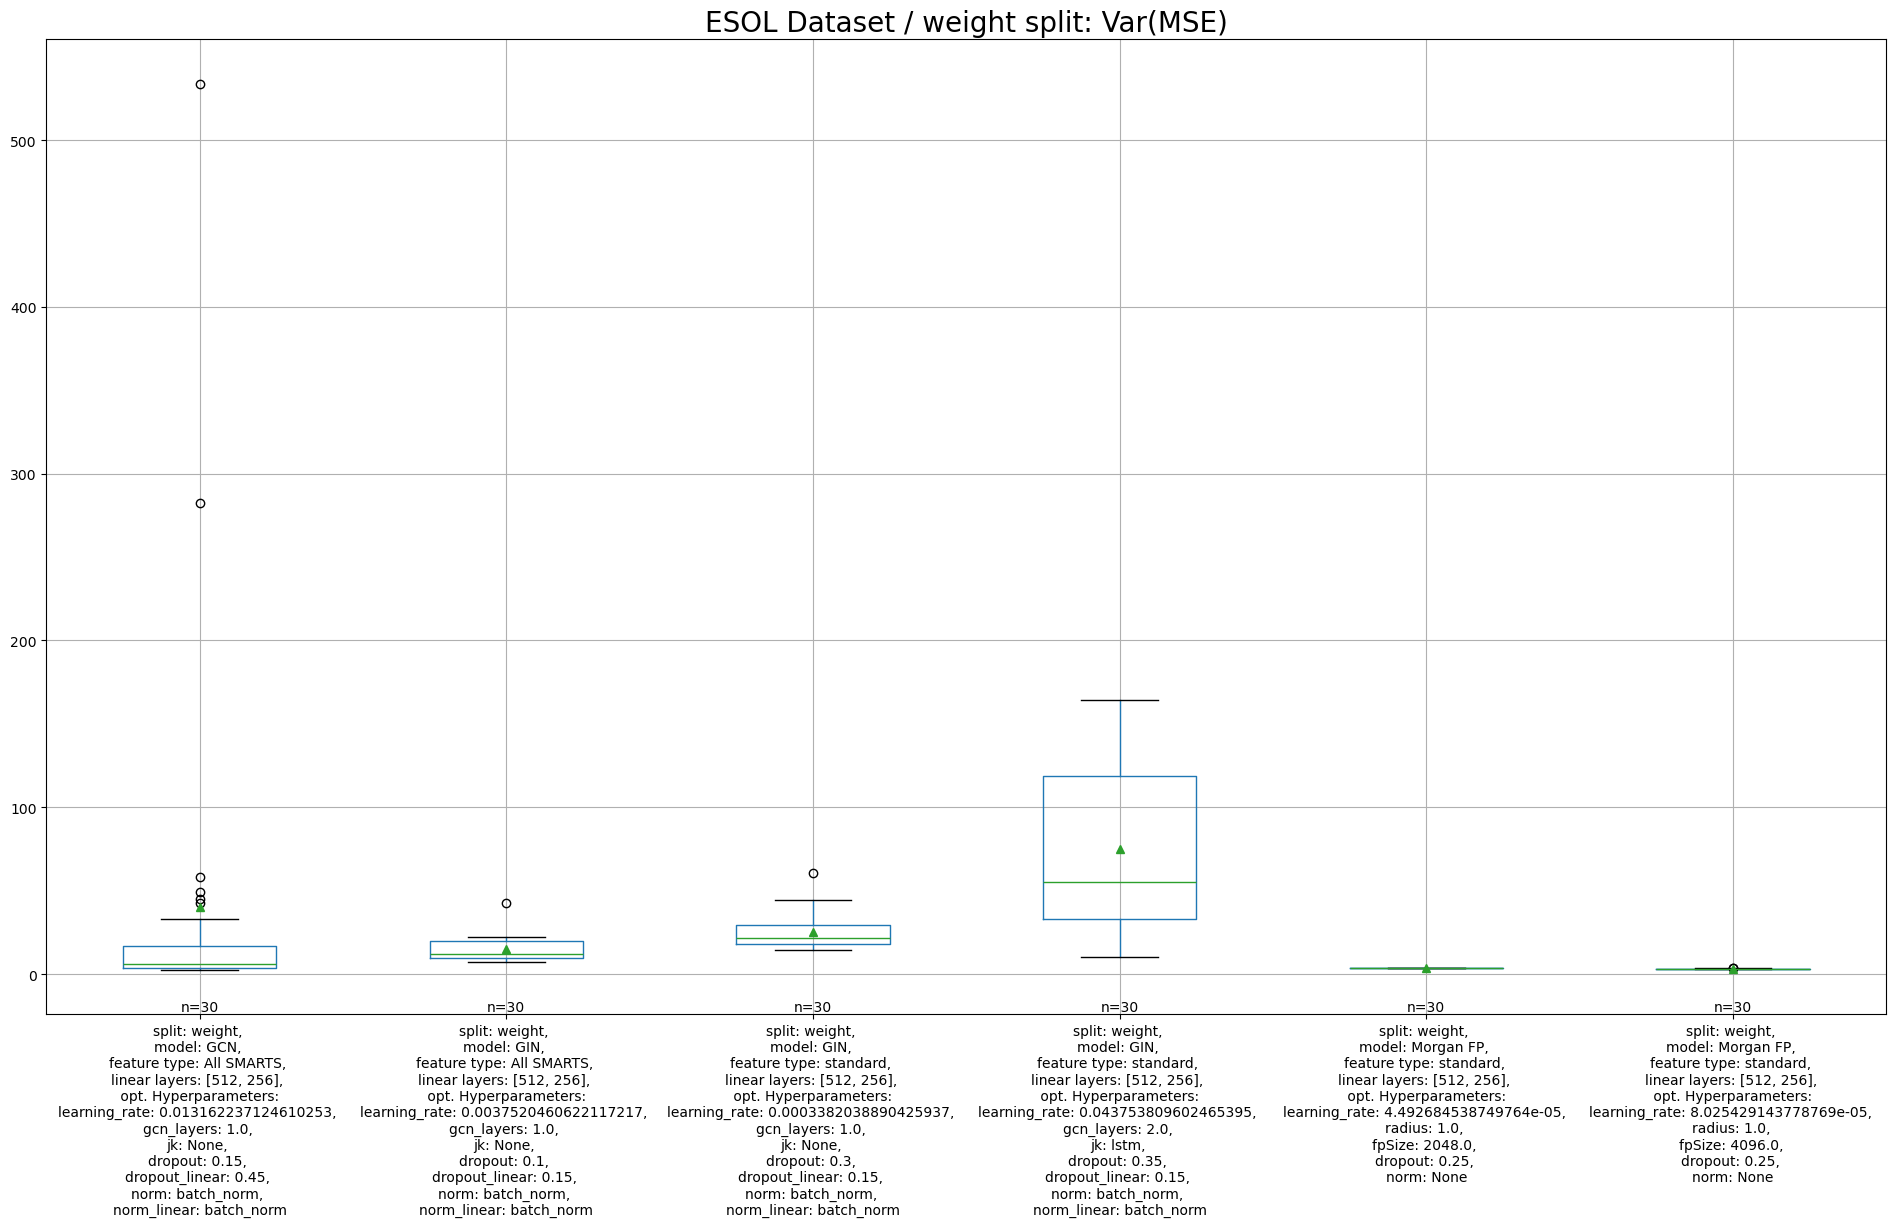
\includegraphics[width=1\linewidth]{weight_split_esol_var_mse.png}
    \caption{Enter Caption}
    \label{fig:weight_split_esol_var_mse}
\end{figure}

Interestingly, it seems that in this case the GIN with frozen layers even performs slightly better.

The combination of all SMARTS strings (the original version from Gobbi and the RDKIT Feature Fingerprint features) give the lowest mean error.


\begin{figure}
    \centering
    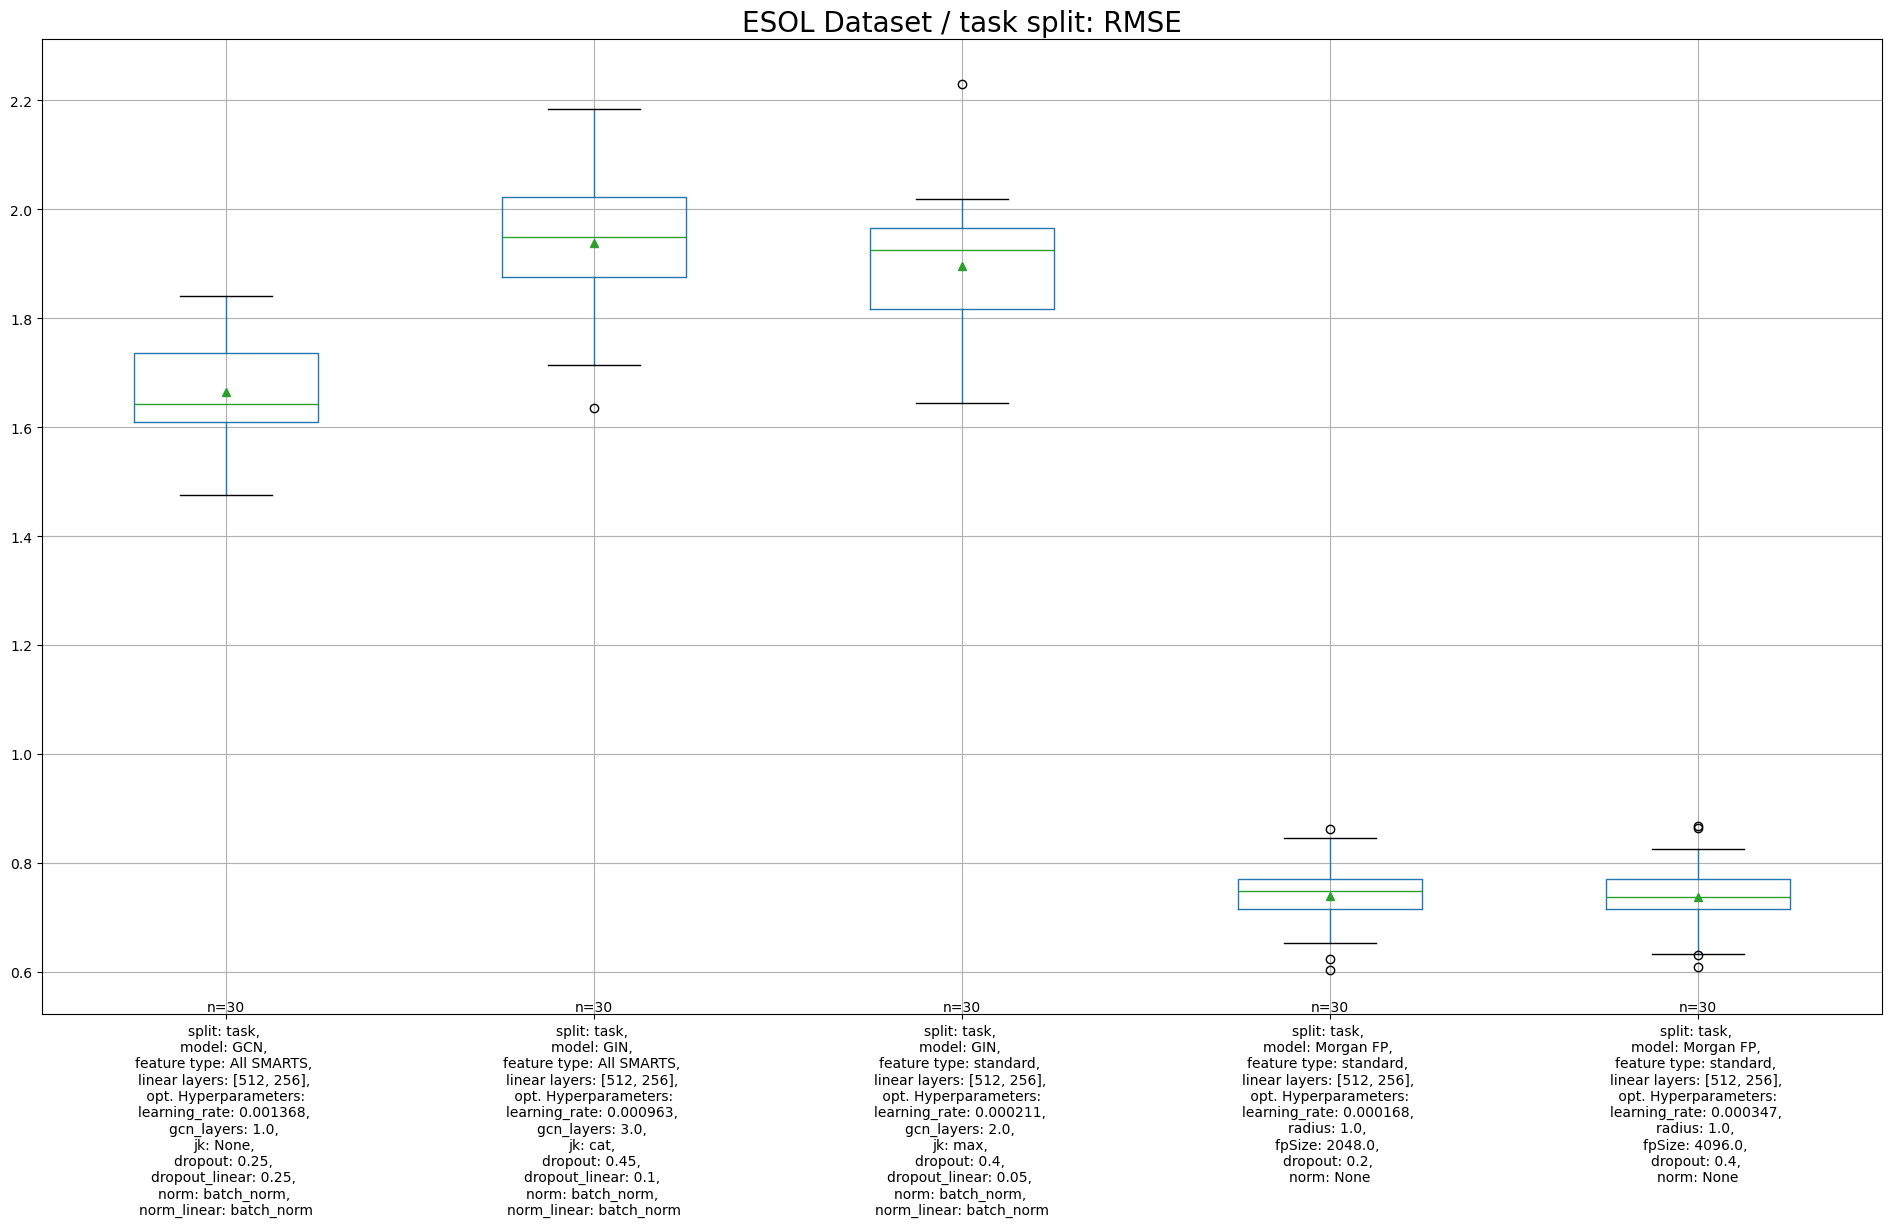
\includegraphics[width=1\linewidth]{task_split_esol.png}
    \caption{Task Split on the ESOL dataset: GCN, GIN and Morgan FP architecture; two runs for Morgan FP}
    \label{fig:task_split_esol}
\end{figure}

\begin{figure}
    \centering
    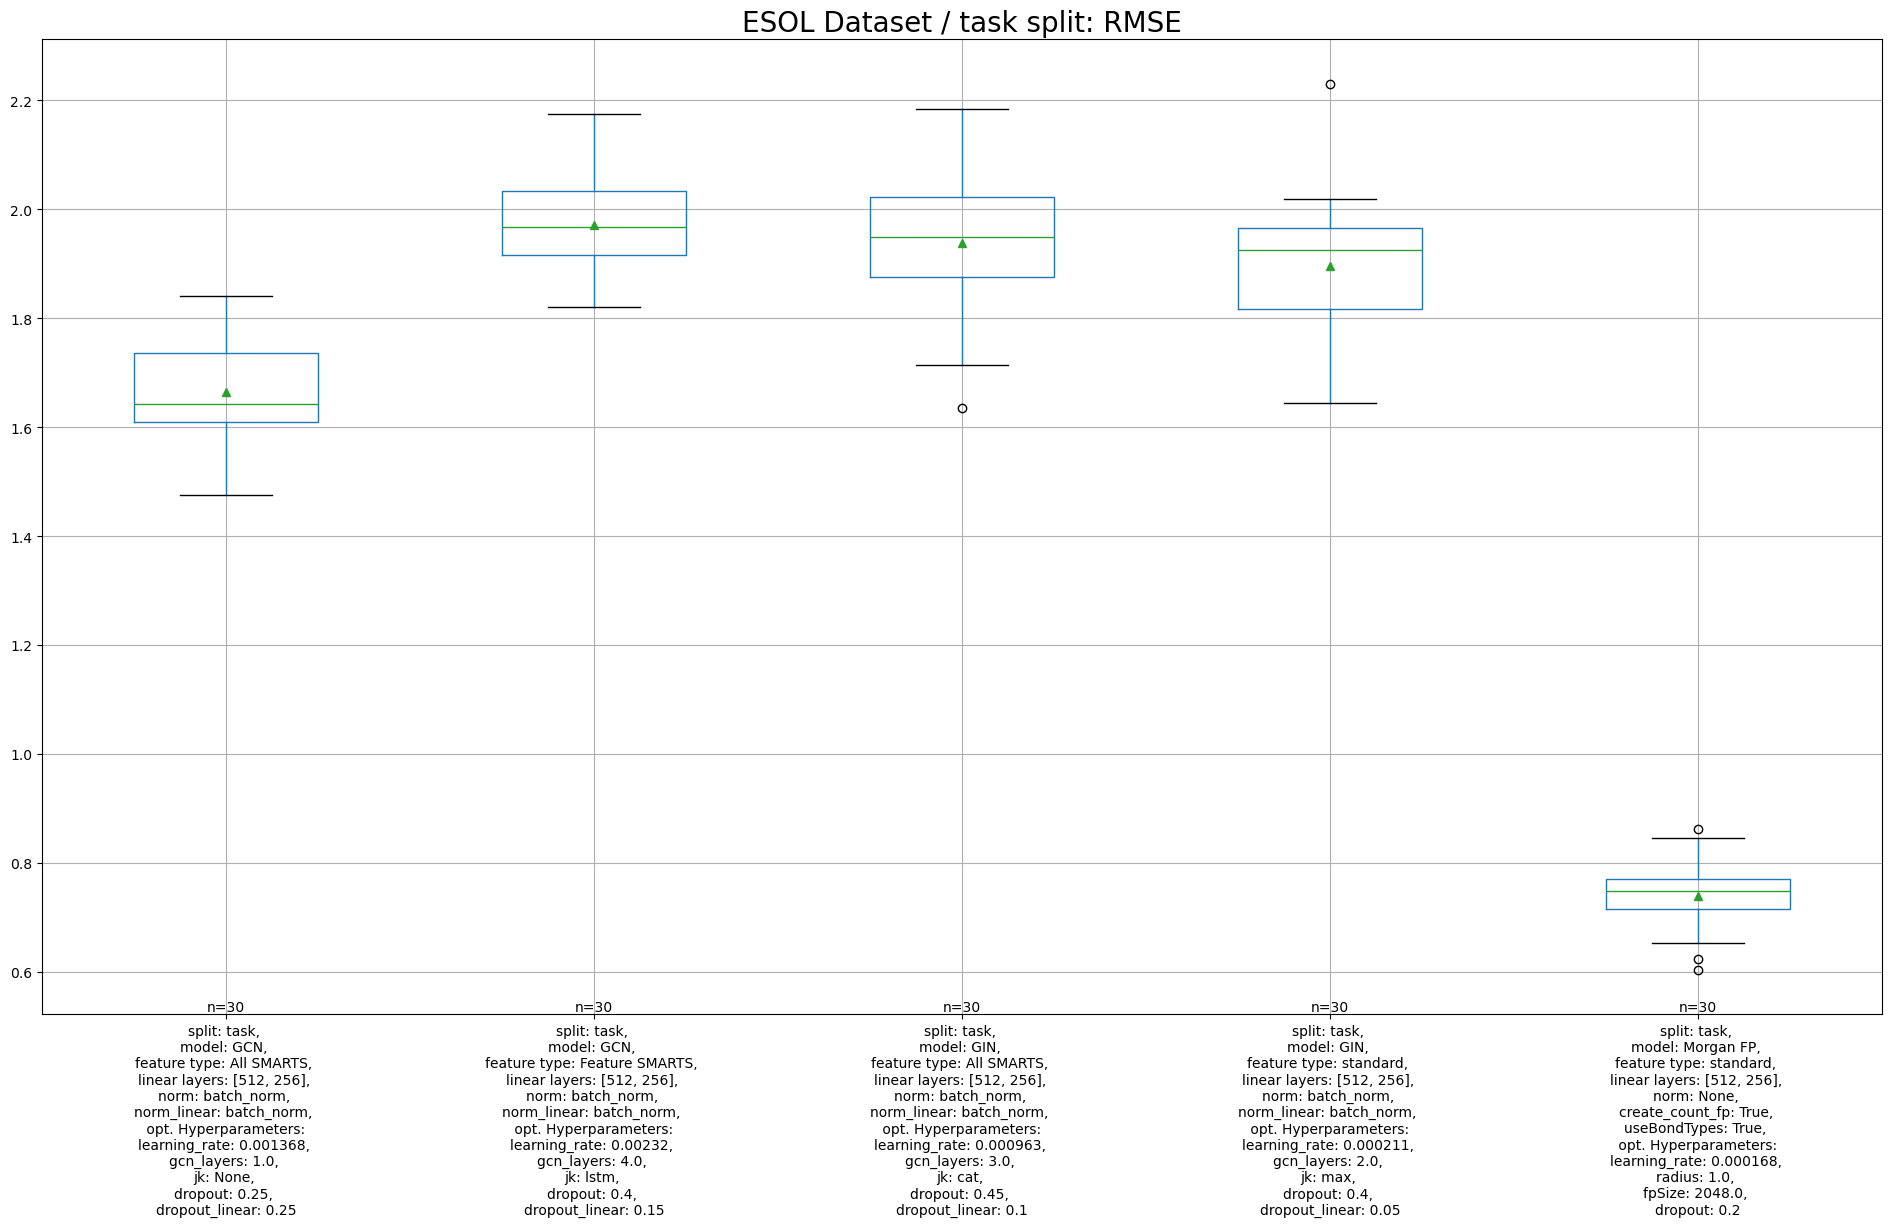
\includegraphics[width=1\linewidth]{task_split_esol_5plots.png}
    \caption{Task Split on the ESOL dataset: GCN, GIN and Morgan FP architecture}
    \label{fig:task_split_esol_5plots}
\end{figure}

For the task split, there are dramatic differences (see fig. \ref{fig:task_split_esol}). Molecular (Count) Fingerprints show a much lower RMSE than graph representations. 


For the splits which reveal tremendous differences between Morgan Fingerprints and GNNs (i.e. task and weight splits), the performance using a combined architecture is of special interest.
On the one hand, such a combination could provide learnable parameters, but also prevent overfitting. On the other hand, it could be that the learnt representation only provides additional noise, indeed leading to a drop in performance.
However, the training process could also simply be able to neutralize these noisy channels and set their weights to zero, effectively eliminating the potential impact of the combined architecture.
Results show that


\subsection{UMAP split on activity datasets}

For the KOR activity dataset, scaffold and UMAP splitting were compared.
Indeed, UMAP splitting leads to a much higher RMSE than scaffold splitting for all classifiers.
However, it should be noted that these values are so high (one can definitely not use these predictions for practical purposes) that one can hardly say that one model is better than the other.

In case of the scaffold split, Morgan Fingerprints perform slightly better than the GNN architectures (correlation plots also show). Correlation plots show that there is almost no positive correlation between these errors.
In contrast to \cite{Zhang.2024}, no consistent difference on the UMAP split could be found.

Again, frozen GIN layers perform significantly worse only when batch norm is applied.

\begin{figure}
    \centering
    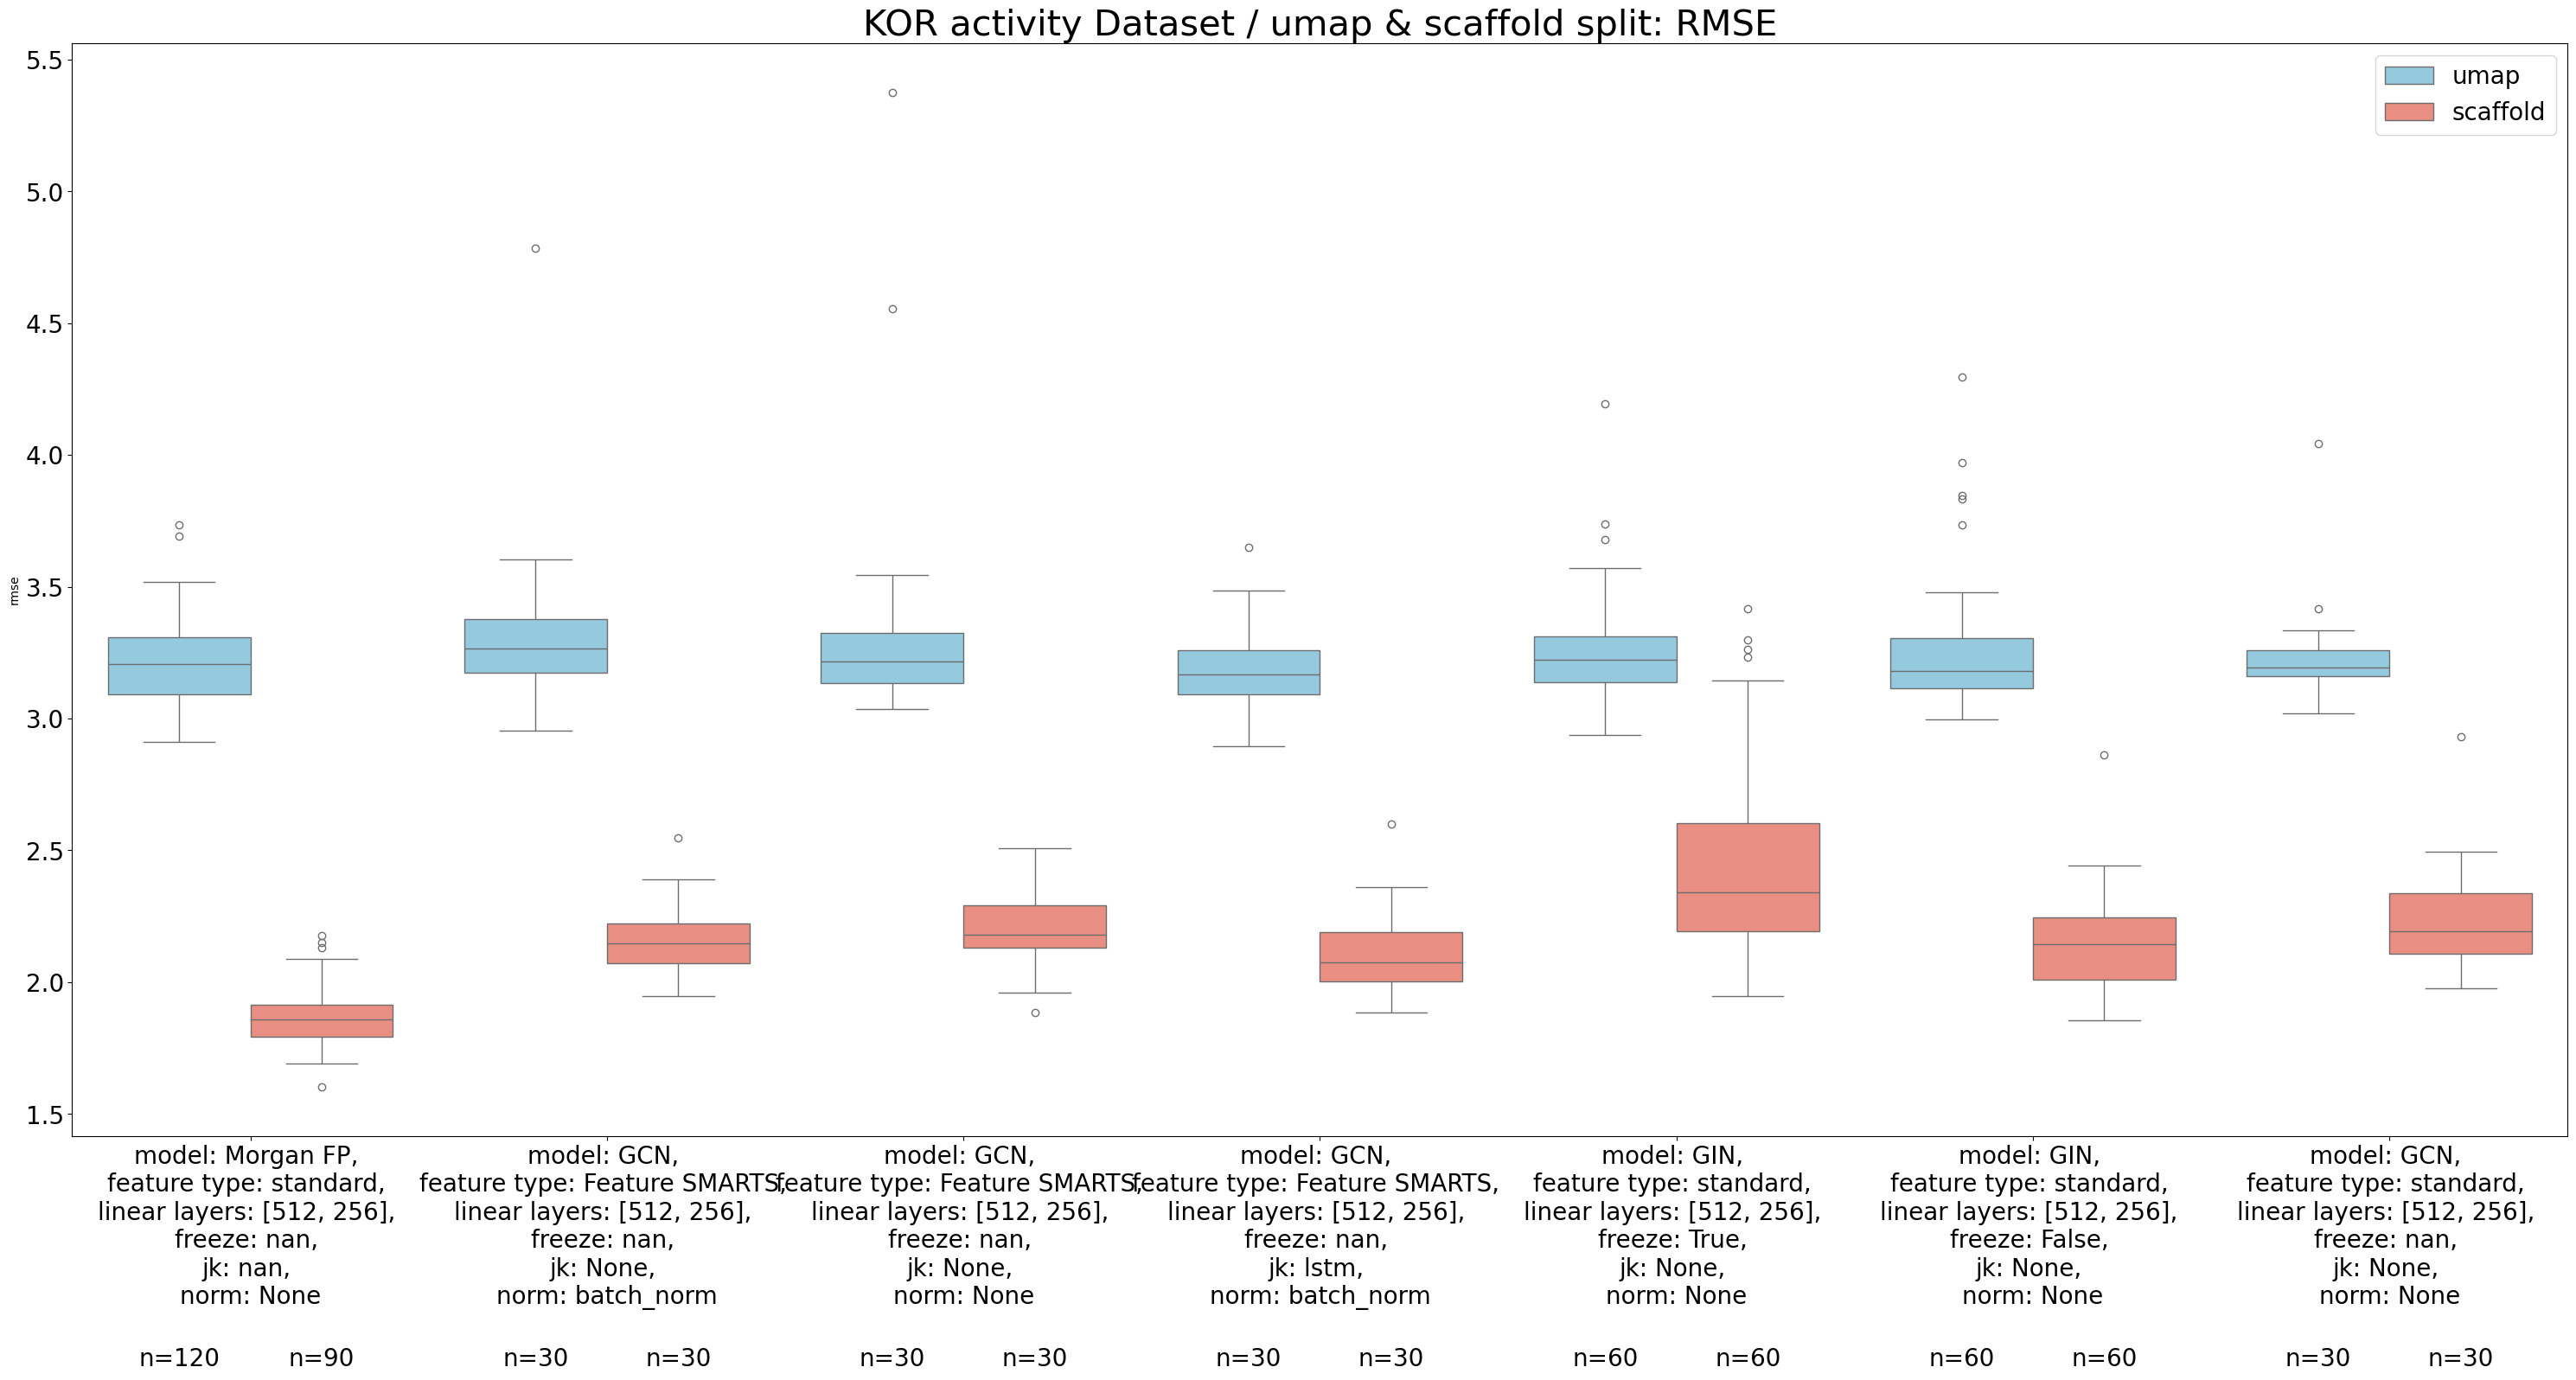
\includegraphics[width=1\linewidth]{umap_scaffold_comparison_kor_activity1.png}
    \caption{Enter Caption}
    \label{fig:enter-label}
\end{figure}

\section{Features and feature representation impact}

For other features, too, the usage of one-hot encoded versions could be more reasonable:

\section{Results for Jumping Knowledge, dropout, combined layers etc.}

The results for Jumping Knowledge are very inconsistent.
In some cases, jumping knowledge modes improve the results slightly, whereas in other variance is increased.

Commonly, batch norm increases performance consistently (except for architectures with frozen layers).
Optimized values for dropout (in the graph part as well as in the classifier) are often very high (even when batch norm is applied), indicating the importance of measures countering overfitting.



\section{Exotic Variations}

Furthermore, some variations of the general architecture consisting of a graph representation, in which atoms are represented as nodes and bonds as edges, and a final dense layer for classification have been tried out.
Even when they do not perform better than the architectures assessed in the previous chapter, a nearer investigations seems to be insightful. 

Similarly, the usage of a complete graph was tried.
Transformer and to the technique of inserting a supernode which is connected to all atoms of the graph representation \cite{Li.12.09.2017} and to the Graph convolution of Weave modules in which features from all pairs of atoms in the molecule are extracted \cite{Kearnes.2016}.

It also seems to be interesting to avoid the bipartite structure of graph representation and final classifier.
The graph channel size is subsequently decreased to 1. Since the output after the final graph layer has already size [1, batchsize], a further classification step is not necessary.

\subsection{Binary networks etc.}

\subsection{Incorporation of global properties}

\section{Custom Loss Functions}

The results so far have confirmed that outliers / activity cliffs play a crucial role.

Given these results, one could experiment with a dynamical version: Depending on the current size of the gradients, the alpha parameter will be modified.

(This is in particular true for some datasets from MoleculeNet which contain entries gathered from multiple publications in which not always the same experimental procedures were applied. This lack of standardization implies that the uncertainty of the reported values is much higher than the inherent error of the experimental setup alone.)


\subsection{Lipophilicity}

The results for the Lipophilicity dataset deviate in an interesting way.

In principle, the performance is very similar, but the lower variance of the GINs suggest their results are more stable. (Which outcome is preferable, depends on the practical purpose.)

Interestingly, in contrast to other datasets, the representation of the features (integer of one-hot encoding) seems to be crucial.

\subsection{Correlation between architectures}

Two related correlations are of interest, the predicted values itself and the residuals. 

Do such uneven splits lead to higher inter-run variance?

\section{Ensemble and Transfer learning}

The low correlation between runs with similar GNN architectures, in contrast to the rather large accordance for Molecular Fingerprints, probably is associated with the high inter-run variance even for the same architecture on the same data: Different runs lead to weight optimization which accurately predicts different data instances. This finding suggests that Ensemble learning, which has proven beneficial in many Deep Learning applications, could improve performance.

Transfer learning yields another opportunity to assess the importance of the trained parameters.
If they are ‚neutral‘, i.e. do not fit tightly to the task, but rather incorporate knowledge about physicochemical properties which can, in connection with an appropriate classifier, be used for different tasks.

(It is clear that this is not fully case: Given that float numbers, the probability is much more smaller. However, one can overcome this problem with the custom activation functions.)
For instance, on e can train it on one dataset use it for another which has the same or a related task.
Datasets which have the same properties (but within a different range), and totally different datasets.

For datasets with multiple properties (e.g., the ADME dataset), one could even try to create combined architectures which were trained on not only the property of interest, but also the other ones.

If GNNs really learn physicochemical properties (which are even of importance beyond the specific task), one should be able to increase performance by such an approach.

The ADME dataset is highly suited for such an investigation, because for many of the compounds several properties are listed, but for only a small subset all data is available.

\subsection{Carbohydrates}


Such compounds which consist solely of carbons (and hydrogens) are of special interest, since in this case the topology remains.
Thus, the layers have been investigated for such examples.


consisting of alkanes and fatty acids of different length.
\cite{Schweidtmann.2023}
Given that binary fingerprints should hardly be able to discern these structures, this is a good check for the reason of performance differences.


\subsection{Influcence of activity cliffs}

prediction error cliffs, i.e. molecules with a very similar objective value, but a high difference in error (for a specific ML/DL model). 

Fig
show interesting differences.

\subsection{Unique mapping of molecules}




\subsection{Subgraph GNNs}

An implementation using pygho has been adopted for the datasets used in this study.

For the ESOL dataset, this gives promising results.

Unfortunately, it is not trivial to adapt the code for processing nodes with multiple features.
    \chapter{Discussion}


\section{Datasets and Performance}


\subsection{Count information and performance}

In particular, count Morgan fingerprints provide significantly better results than bitwise fingerprints. There was no case found in which bitwise fingerprints show better performance, but the size of the difference is highly different depending on the dataset. In most cases, it is rather moderate, but in particular for the ESOL dataset, it is huge.
For this superiority of count- over bitwise-fingerprints, the explanation is simple:
In the ESOL-dataset, molecules with a high number of identical substructures are common.

(even with a radius size of 4, they cannot be distinguished).

This leads to the problem that fatty acids of different chain length cannot be distinguished anymore.

The ESOL dataset contains a lot of fatty acids and related compounds and it is known that the target property, solubility, is highly negatively correlated with the length of fatty acids.



It would be insightful which (generalized) similarity values GNN architectures get for these compounds.


\section{Feature selection and Performance}

Interestingly, despite the differences between ECFP-like Morgan fingerprint and feature fingerprint are very small and in general no fingerprint is superior to the other, the involved features perform differently used as input for a GNN.


The results also show how much the optimal parameters, e.g. for the number of layers and the hidden channel size, differ (however, one should keep in mind that regularly multiple parameter combinations give equally good results). This puts many of the results published previously into perspective.
E.g. in \cite{Deng.2023}, for the performance of GIN and GCN a much worse performance was reported than found in this study (in which they outperform binary fingerprints and are on equal footing with count fingerprints).
Given the results of this study, the settings in \cite{Deng.2023} were severely biased against GNNs (in contrast to other studies like Duvenaud et al. 2015 which reported a superiority of graph representations solely because of the suboptimal fingerprint).
(Of course, for practical purposes one has to keep in mind that the determination of optimized (hyper-)parameters can be a very costly process in terms of time and computational resources.) 

On the other hand, hyperparameter optimization of GNNs was not done in-depth, but a default setting with an embeddings size of 300, a hidden channel size of 512 and 5 layers has been used.

For instance, in \cite{vanTilborg.2022}, all models were trained for 300 epochs and the early stopping patience was set to ten epochs, which arguably is a very low number in this setting (also given the fact that most datasets are not very big), possibly excluding good solutions.

By taking a different fingerprint for splitting, one could potentially create datasets which are neither biased against one of the compared representations.

This also explains why the effect of the encoding of the features (integer or one-hot-encoding) affects the performance differently depending on the dataset. For some datasets, in particular the solubility related, properties like the molecular weight which can be directly evaluated from the atomic number is of high importance, whereas in other cases, the extraction of the meaningful features from the integer value is very difficult, but the one-hot-encoding allows that a particular atom type is associated with a specific weight.


Recently, the problem with scaffold splitting was reported in another study \cite{Zhang.2024}.
These findings have been confirmed.


\cite{Comparison of fingerprint and GNN performance}

One should again stress the fundamental difference between circular fingerprints: Due to its learnable parameters, GNNs can adapt to the current task; exactly this task-awareness potentially also leads to overfitting to the training data. 
On the other hand, Morgan fingerprints only rely on the fixed, task-agnostic substructures which – so could be argued -, also maintain some predictive power out of distribution.

Performance differences between fingerprints 
This can be highly misleading, indicating that there is no significant difference between fingerprint and GNN predictions as seen on the ADME datasets.

Furthermore, the focus on the magnitude of the error (e.g., RMSE) regularly conceals crucial differences, e.g. in the variance or the distribution of the errors. Indeed, for various datasets it was confirmed, although the mean error is about the same, the variance of the error between runs is even of different order of magnitude.


(Additionally, it should be noted that different hyperparameter settings can lead to different results. In particular for the frequent case that the performance difference between the architectures is not very large, the choice of the parameters can easily alter the ranking of performance.)

For a given dataset, GNNs are much more sensitive to the split technique or different subset selections.

The problem for unequal densities in the case of GNNs for regression tasks is tightly related to the imbalanced datasets for classification.


Advanced splitting techniques show that an unbiased performance comparison between molecular fingerprints (e.g., coupled to a DNN as classifier) and a graph representation (as well using a DNN) is much more complex.

Weight and task-specific splits reveal much bigger differences.

For limited training data, the likelihood that there are serious gaps in the distribution of the objective values is much higher etc.


\section{Splits and Performance}

Scaffold splitting is a recommended split technique for the discovery of new potential categories (for this reason, it is recommended, e.g., for the HIV dataset).

Whereas for random splitting the ratio should be on average equal to the full dataset, other splitting techniques can highly distort it.
For regression tasks, the problem is similar: Depending on the split, the distribution can significantly differ.

(The problem is - in particular in the context of activity cliffs - that high compound similarity clearly positively correlates with 
(There are of course exceptions, in particular when bitwise fingerprints are used in combination with a small radius: In this case, 'identical' - i.e. Tanimoto similarity of 1 - compounds can differ highly on specific values, for example solubility.)


\section{Investigation of frozen layers}

Interestingly, for most datasets, frozen GIN layers provide much worse results when coupled with batch normalization.

, i.e. a typical case of oversmoothing.

The effect of frozen layers has been analyzed checking Tanimoto similarity and layer outputs.
Batch normalization reduces the variability, giving rise to the counter-intuitive result that for frozen layers it worsens performance.



For the Morgan Fingerprints, the difficulties are less pronounced; however, also in these cases the outcome of hyperparameter optimization runs can differ significantly (examples are shown in the results).



For comparison of the architectures, it is not only important to know how large the differences in terms of the error are, but also whether the same instances are giving rise to high errors, i.e. the correlation between the outcomes.

This behaviour is greatly amplified by irregular splitting techniques.

In many cases, variance is much higher for architectures using graph representations. Whereas runs with the optimized FPN give almost identical results, there is a wider range for all graph representations.

On well-known datasets (e.g., ESOL) it was demonstrated that the splitting technique highly influences the performance differences between the architectures. Further results have shown that this finding can be generalized.


From this perspective, the GNN architectures also could forget structures which are not of importance for the task at hand, leading to better generalization.

However, it should be noted that the performance increase for feature-based fingerprints and feature subsets is limited. Depending on the task, also pharmacophore-based fingerprints could be used etc.

	\chapter{Conclusion}

In this thesis, mostly basic graph neural network architectures were analysed. This was due to the goal of comparing classical fingerprints as directly as possible to neural networks.
However, it would be interesting to extend the investigation to other architectures like GAT and more complex MPNN-based architectures or also compare the performance of pretrained models like MolBERT.

In this regard, it would also be tempting to investigate more sophisticated training routines, i.e. 
and in the later epochs train specifically with activity cliff data.

For instance, one could alter the activation function (either change it or modify the alpha-parameter of the scaled ones) during training.

For this study, the Morgan fingerprint was used due to its simplicity and, above all, its similarity to the operations (like convolutions) which are applied in graph neural networks.
Furthermore, it would be interesting to include other fingerprints (e.g. MACCS) and compare their performance. 

I also should be noted that also other types of fingerprints exhibit similarities, i.e. Daylight fingerprints working on subgraph representations of the molecule.

The contradictory results in previous studies often can be traced back to the application of different implementations, e.g. the Neural Fingerprint presented in Duvenaud et al. 2015 is indeed superior to the binary Morgan fingerprint on the ESOL dataset, but it is outperformed for the count-based version. 

This leads to the idea that a task-specific feature extraction step (which could either be based on background knowledge, classical Machine Learning or an additional Deep Learning architecture) combined with a graph representation approach could improve results significantly.

It also should be noted that even the analyses shown did not vary all possibly important parameters, i.e. the aggregation function used in the Message Passing step. One could also experiment with adaptive learning rates and more sophisticated loss functions.

On the other hand, similar to baselines like linear regression and the prediction solely from global, unspecific properties like molecular weight, one should also bear in mind that the existence of an upper limit cannot be ruled out.

Furthermore, the problem of splitting has been exposed in an unprecedented way.
It was observed that the performance differences between architectures can be maximized for specific splits.

Reliance solely on random and scaffold splits falsely suggests that Morgan Fingerprints and GNN architectures are equivalent, whereas other splitting techniques show that there are large differences.

A major contribution of this thesis was the usage of the RdKit feature Morgan-Fingerprint features (which are originally conceived in Gobbi 1999) as input for a GNN. 
(For instance, it can be argued that the atomic number is a bad feature: Of course, it linearly correlates almost perfectly with the atomic weight, but chemical properties cannot easily deduced because they rather depend on the group in the periodic table.)

Interestingly, severe biases against fingerprints as well as graph-representations have been found in the reviews and publications proposing new Deep Learning models for molecular property prediction.

For performance improvement, methods beyond dropout and normalization should be employed.


Furthermore, it can be confirmed that benchmarks and performance assessments of new models should not rely only on typical benchmark datasets like MoleculeNET, but should, e.g., also incorporate custom datasets created from ChEMBL, ZINC or other sources.






It should be noted that there is no training of the graph involved, all parameters are frozen.

\begin{itemize}
\item	Various methods of transforming a graph neural network representation into a fingerprint as similar as possible to the Morgan fingerprint have been conceived.
\item	The performance on various datasets has been explored.
\item	In particular,
\end{itemize}



As noted initially, mostly rather basic models were compared.

However, the results also indicate that with proper hyperparameter optimization the selection of the best model even becomes more difficult.

    
	%add your sources in the bib file and change the style here
    %\bibliographystyle{alpha}
    \bibliographystyle{unsrt}
	\bibliography{bibliography,activity_cliffs,GNN_mol_fp,gnns,admixture2,additional_bib,subgraphs,binarynn,fingerprints}
	
	\printglossary[type=\acronymtype]
    \printglossary

    \cleardoublepage{}
	\pagebreak
	
	%add your end matter here
	%\appendix{}

	%\input{C) Back Matter/appendix}
	
	
	
\end{document}